\clearpage
\chapter{Physics Object Definitions}\label{sec:objects}
%reconstruction algorithms, isloation, cleaning, IDs, particle flow

This section provides the definitions of physics objects used in the analysis.
The analysis uses two main CMS reconstructed objects: muons and jets.
Photons do not show anywhere in our signal process.
$\tau$'s of our signal process can decay into electrons with the same probability as into muons.
However, the analysis uses b-parking and only targets the muon decay mode of the $\tau$.
Electrons are not an interest of our analysis either.

Although the signal's final decay involves $\tau$ lepton, we do not use CMS reconstructed $\tau$.
Given that $\tau$ decay results in many different objects (muon, electron, and different combinations of hadrons) as shown in figure \ref{fig:tdecay}, CMS uses a special reconstruction algorithm for $\tau$ object.
Particle-Flow jets (PFjets), with all particle identification information within the jet, are the starting point for the $\tau$ reconstruction.
With $\pi^{0}$ reconstructed in ECAL as a strip, the Hadronic-Plus-Strip (HPS) algorithm reconstructs $\tau$ (at 60\% efficiency in Run 1) when a charged hadron and a strip are reconstructed in the PFJet \cite{HPS}.
Therefore, CMS reconstructed $\tau$ collection only includes hadronically decayed $\tau$ lepton.
One of our signal process tau lepton decays into muon, in a leptonic mode, for the trigger.
Although other tau lepton could still decay hadronically, usage of CMS reconstructed tau leptons in the analysis would be accompanied by a division of several different sub-channels (muon, electron, had), which result in 27 ($3^{3}$) different combinatorics.
Thus, we approach a tracker-oriented method with regions of interest to analyze other tau leptons in the signal process.

We use muons, jets, and only tracks (ROIs) for this analysis.
\section{Muons}\label{sec:muons}
The analysis sources the ``SlimmedMuons'' collection from the MINIAOD MC datasets to produce {\tt selectedPatMuons}.
Muon objects are required to have 
\begin{itemize}
  \item \pt $\geq$ 12\GeV to reach B-Parking trigger plateau
  \item $|\eta|$ $\leq$ 1.5 for L1 seed $|\eta|$ cut in B-Parking trigger
  \item reco::Muon object matched to the B-Parking trigger object
  \item Pass the Loose ID criterion (isLooseMuon) as described in the Muon POG~\cite{muonpog}.
\end{itemize}

\begin{figure}[h!]
  \caption{Data/MC of muon objects \pt, $\eta$, energy, nMu}
  \label{fig:muons}
  \centering
  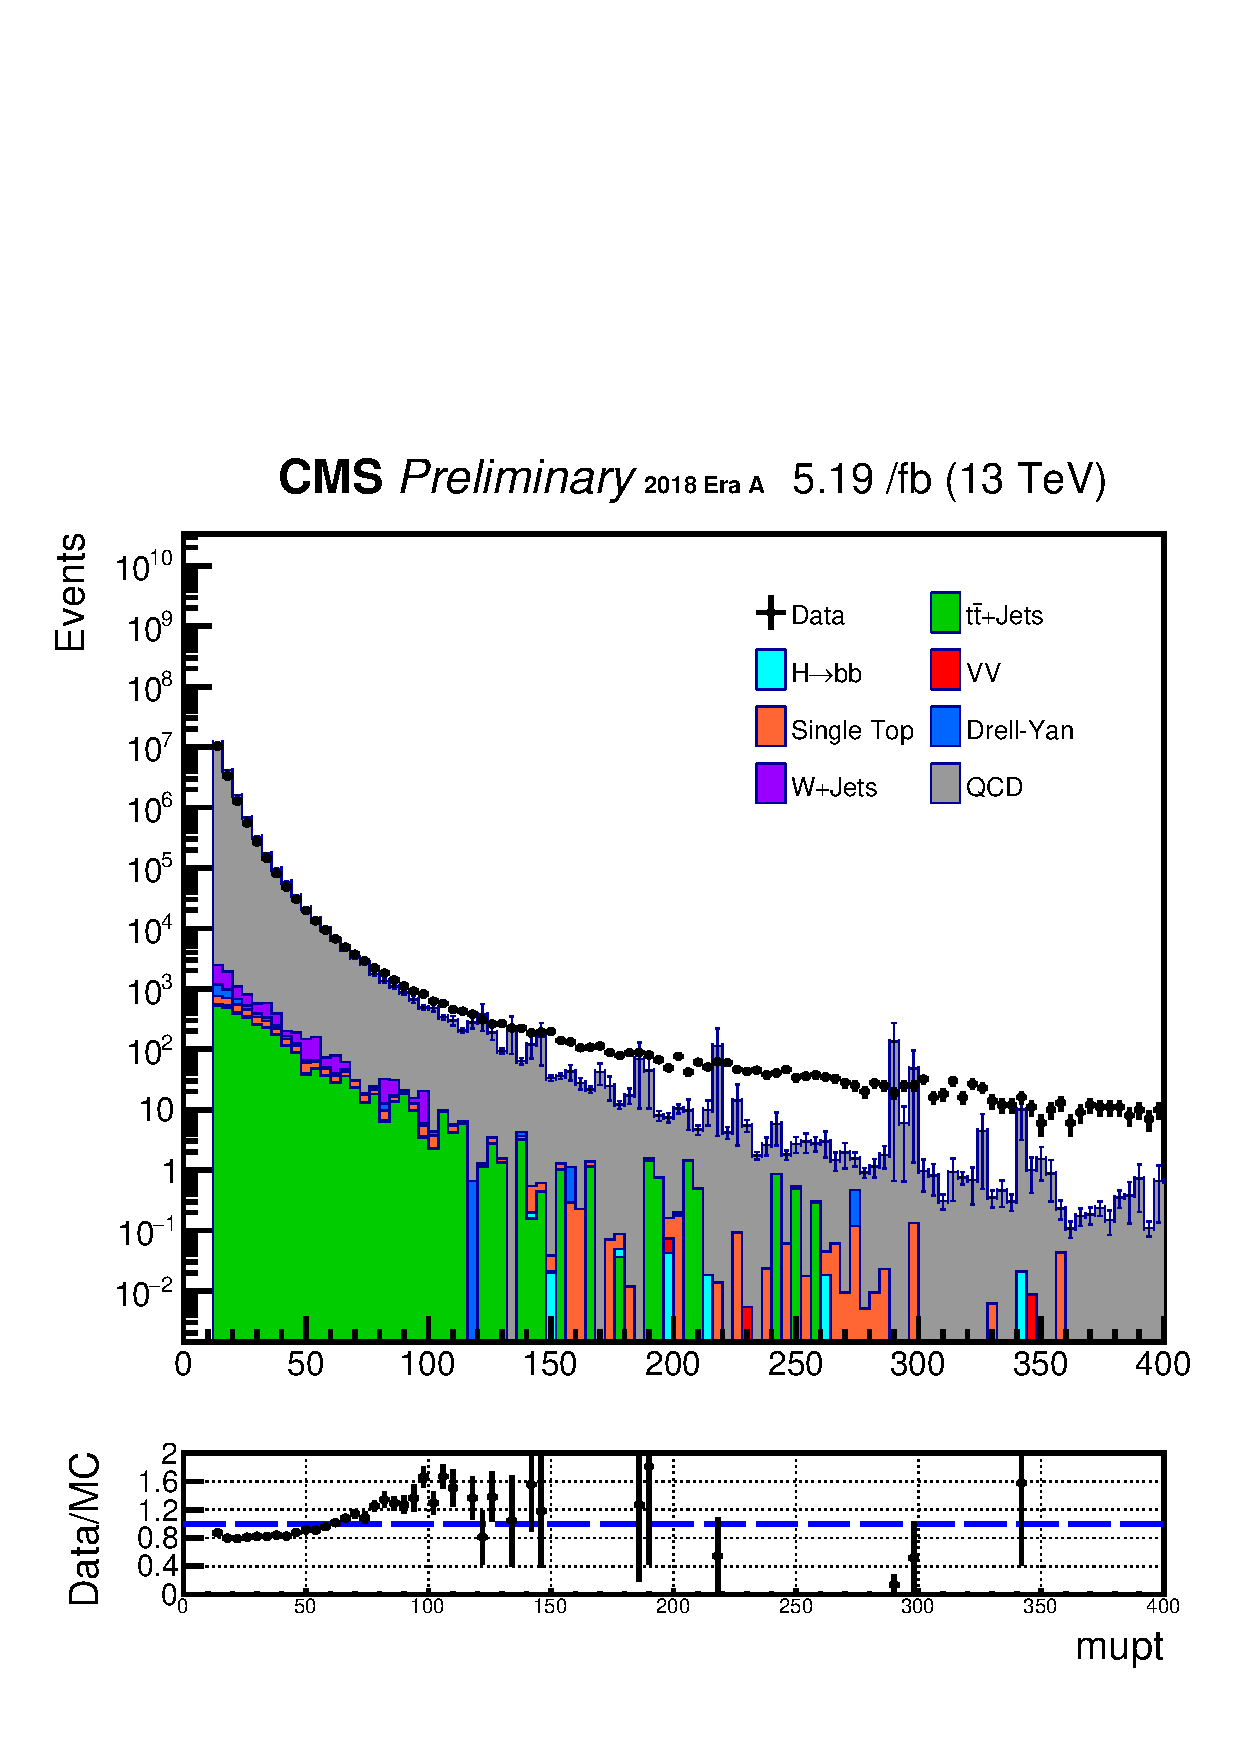
\includegraphics[width=0.47\linewidth]{figs/Data_log_AnalysisNote_MS-15_ctauS-10_mupt.pdf}
  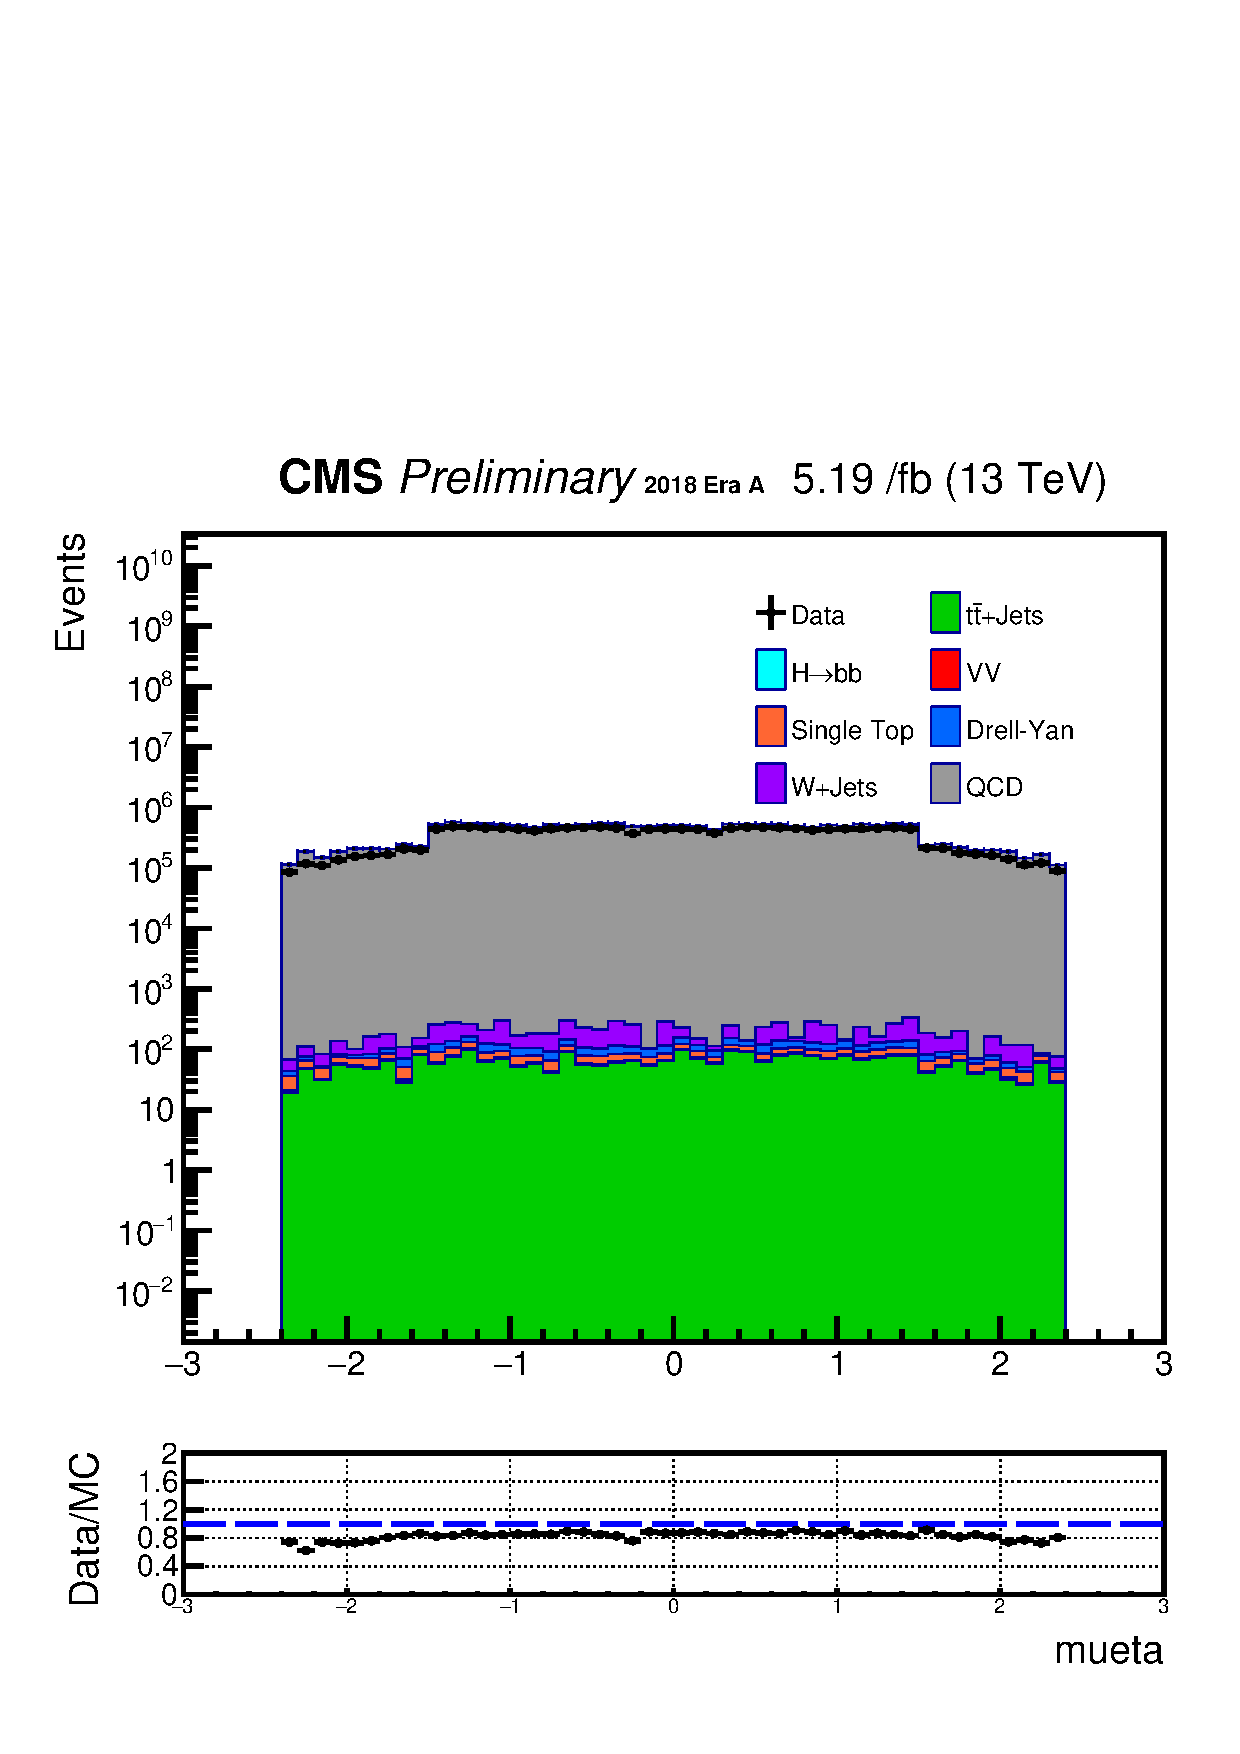
\includegraphics[width=0.47\linewidth]{figs/Data_log_AnalysisNote_MS-15_ctauS-10_mueta.pdf}
  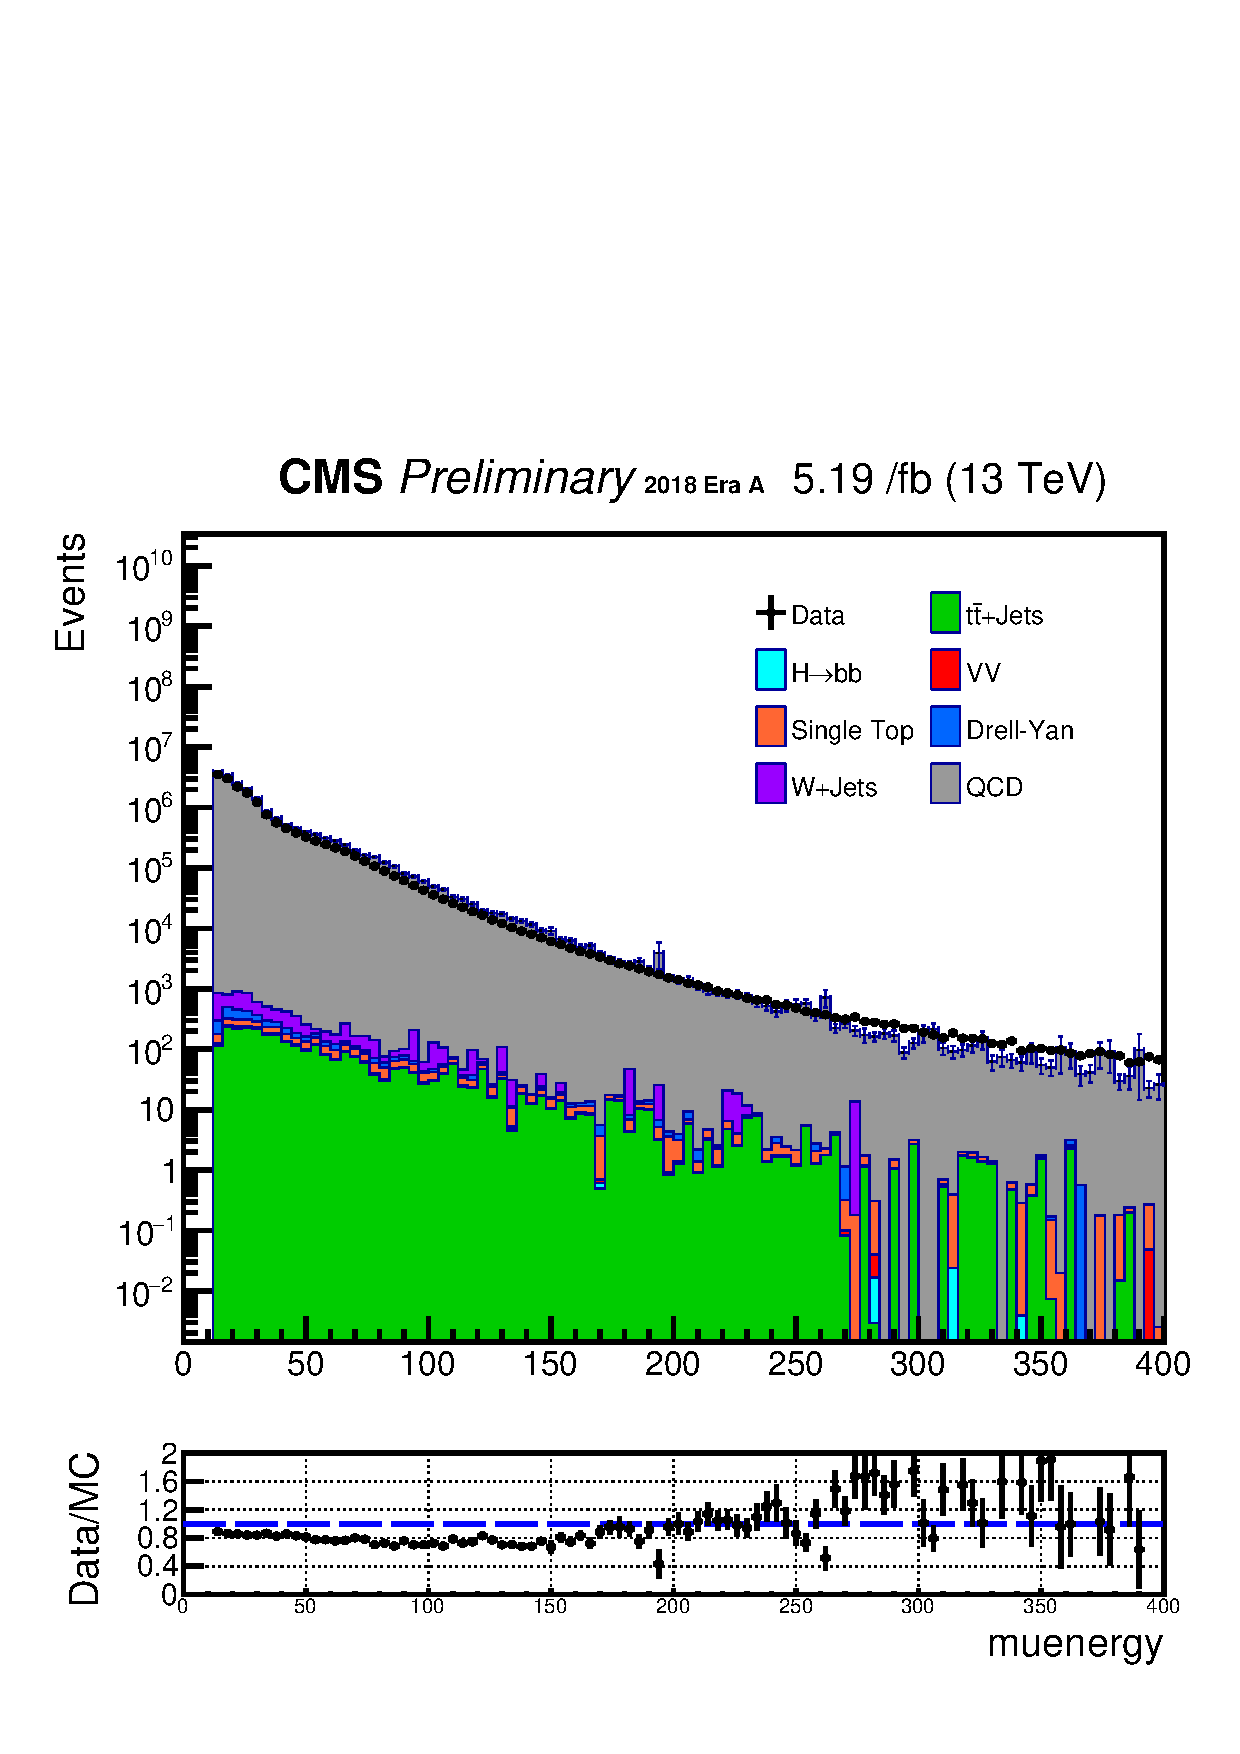
\includegraphics[width=0.47\linewidth]{figs/Data_log_AnalysisNote_MS-15_ctauS-10_muenergy.pdf}
  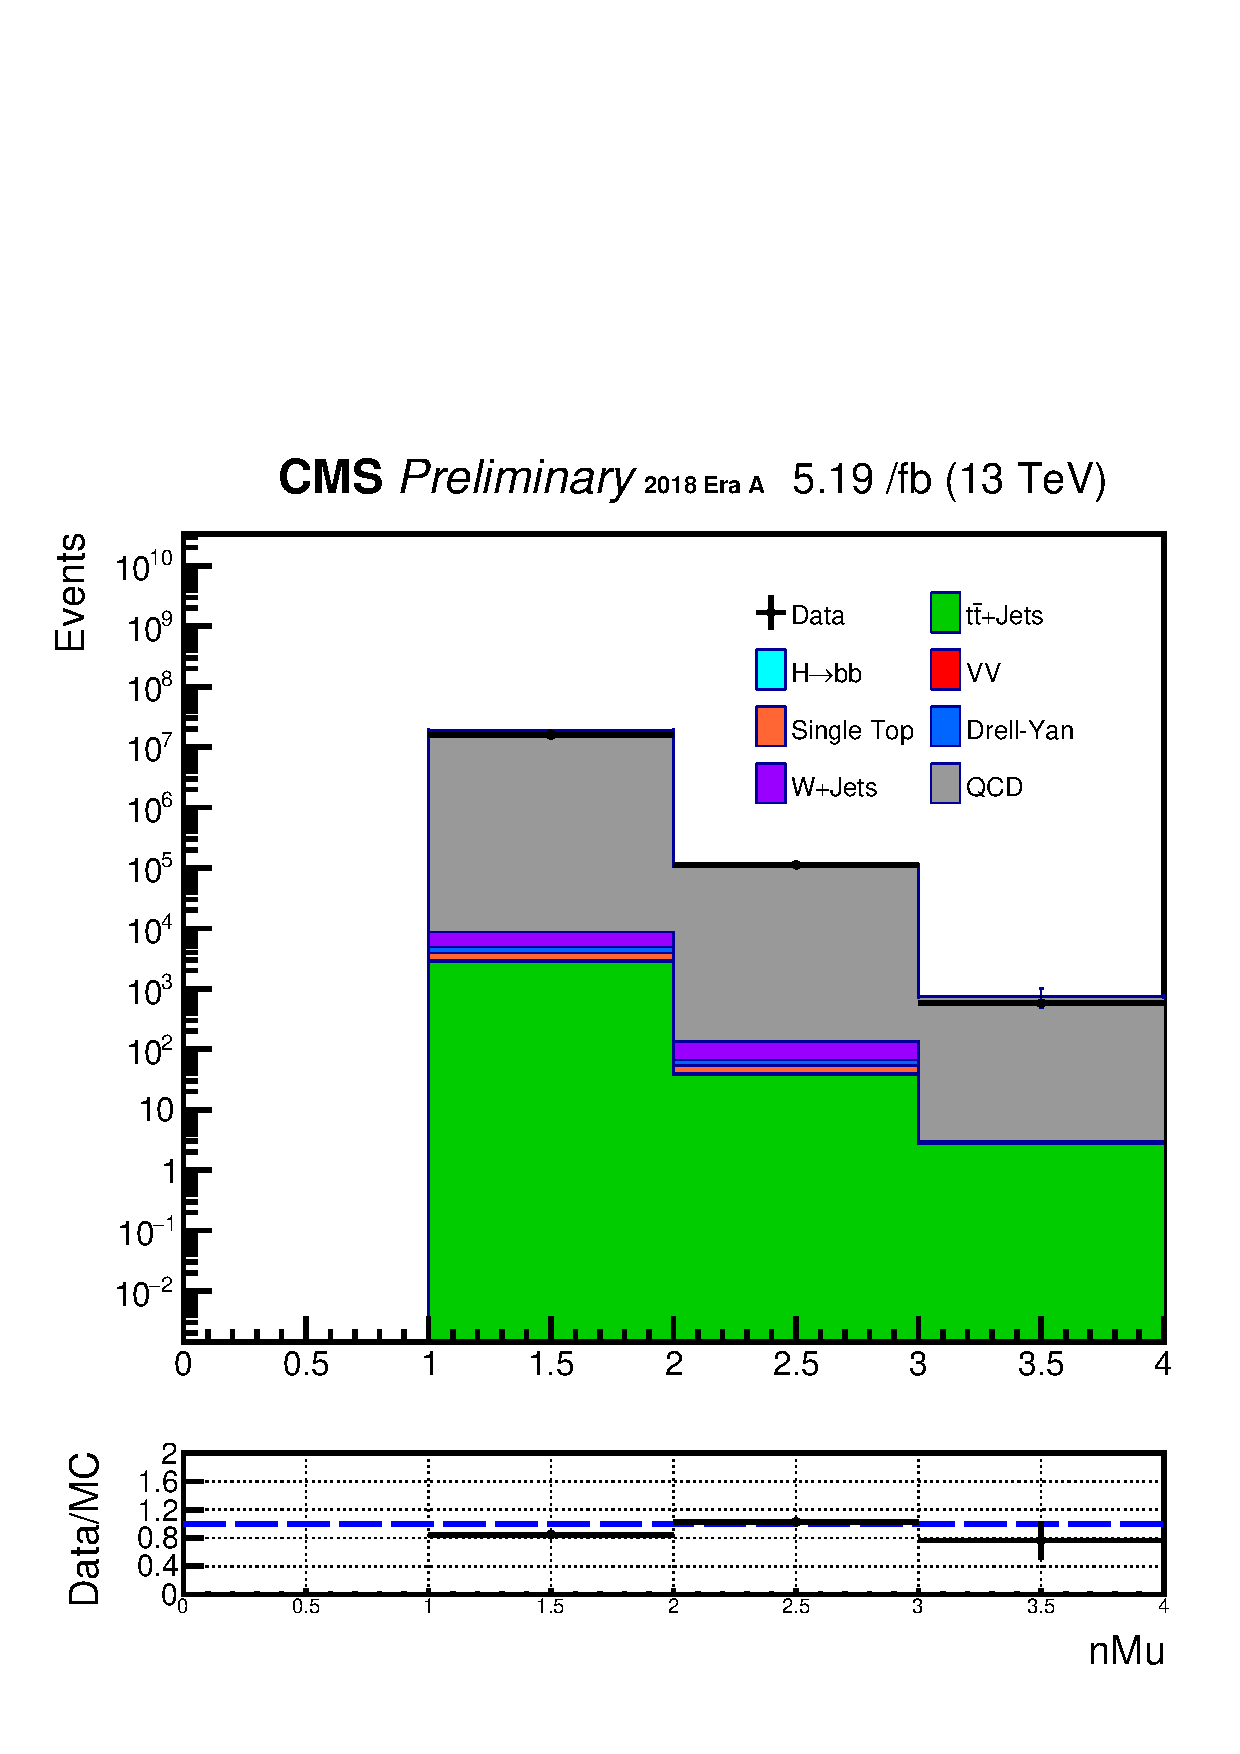
\includegraphics[width=0.47\linewidth]{figs/Data_log_AnalysisNote_MS-15_ctauS-10_nMu.pdf}
\end{figure}

The motivations for isolation requirements on muons are further discussed in Section~\ref{sec:selections}.


\section{Jets}\label{sec:jets}
The analysis sources ``SlimmedJets'' collection from MINIAOD dataset to produce {\tt selectedJets}.
CMS reconstructs jets from calorimeter energy deposits using the
anti-$k_T$ clustering algorithm with a distance parameter of $R=0.4$~\cite{Cacciari:2008gp}.
Then, the calojets are input into the Particle-Flow (PF) algorithms to produce the PFJets collection. Then, variables in PFJets class are slimmed to be saved into MINIAOD files.
%The analysis uses these SlimmedJets for the jets' b tagging scores as well.
Jet objects require
\begin{itemize}
  \item \pt $\geq$ 20\GeV
  \item $|\eta|$ $\leq$ 2.4
  \item 0 $\leq$ emEnergyFraction $\leq$ 0.9
  \item 0 $\leq$ energyFractionHadronic $\leq$ 0.9
  \item No selected electron or muon within $\Delta R=0.4$
\end{itemize}
The energy fraction cuts above are taken from the recommended Run2 Tight jet ID
cuts for particle flow jets~\cite{jetid_2018}.
\begin{figure}[h!]
  \caption{Data/MC of jet objects for \pt, $\eta$, energy, nJet}
  \label{fig:jets}
  \centering
  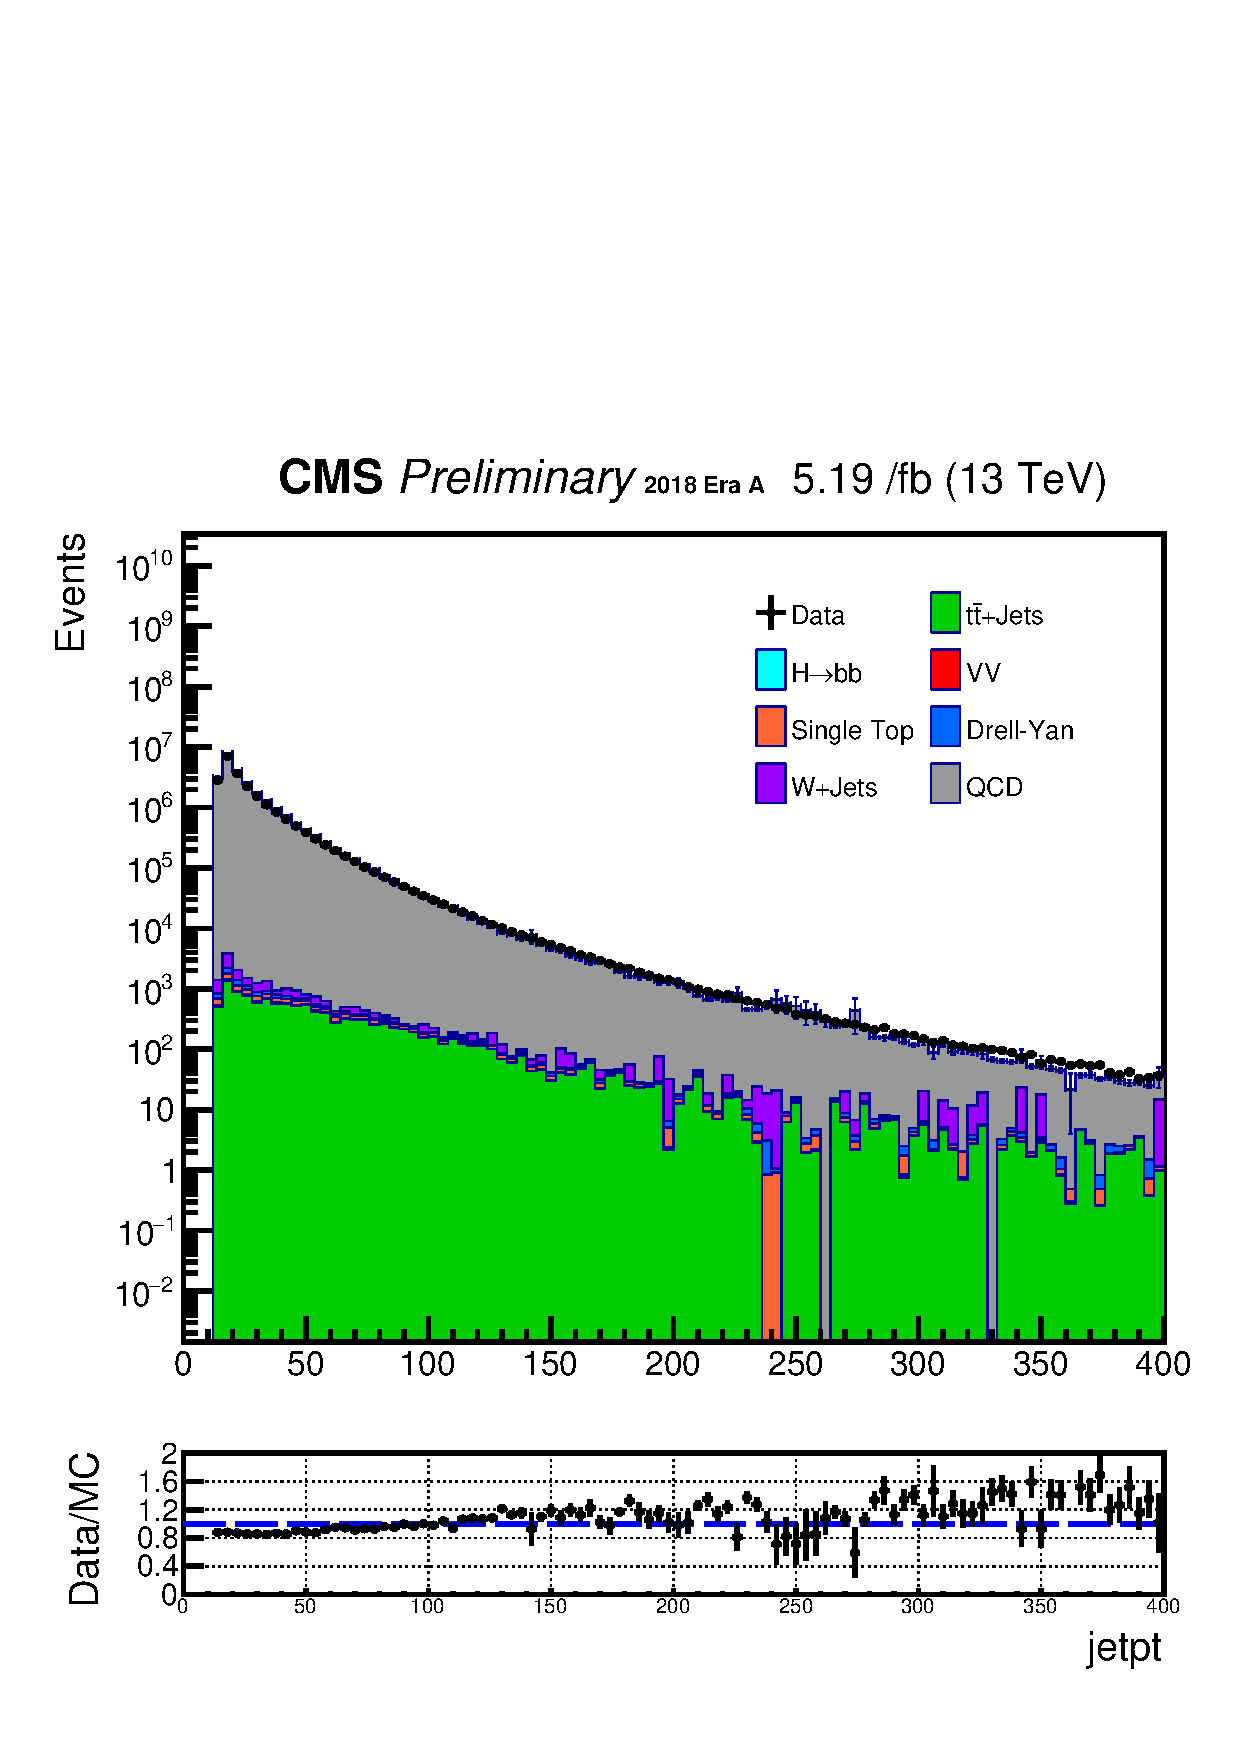
\includegraphics[width=0.47\linewidth]{figs/Data_log_AnalysisNote_MS-15_ctauS-10_jetpt.pdf}
  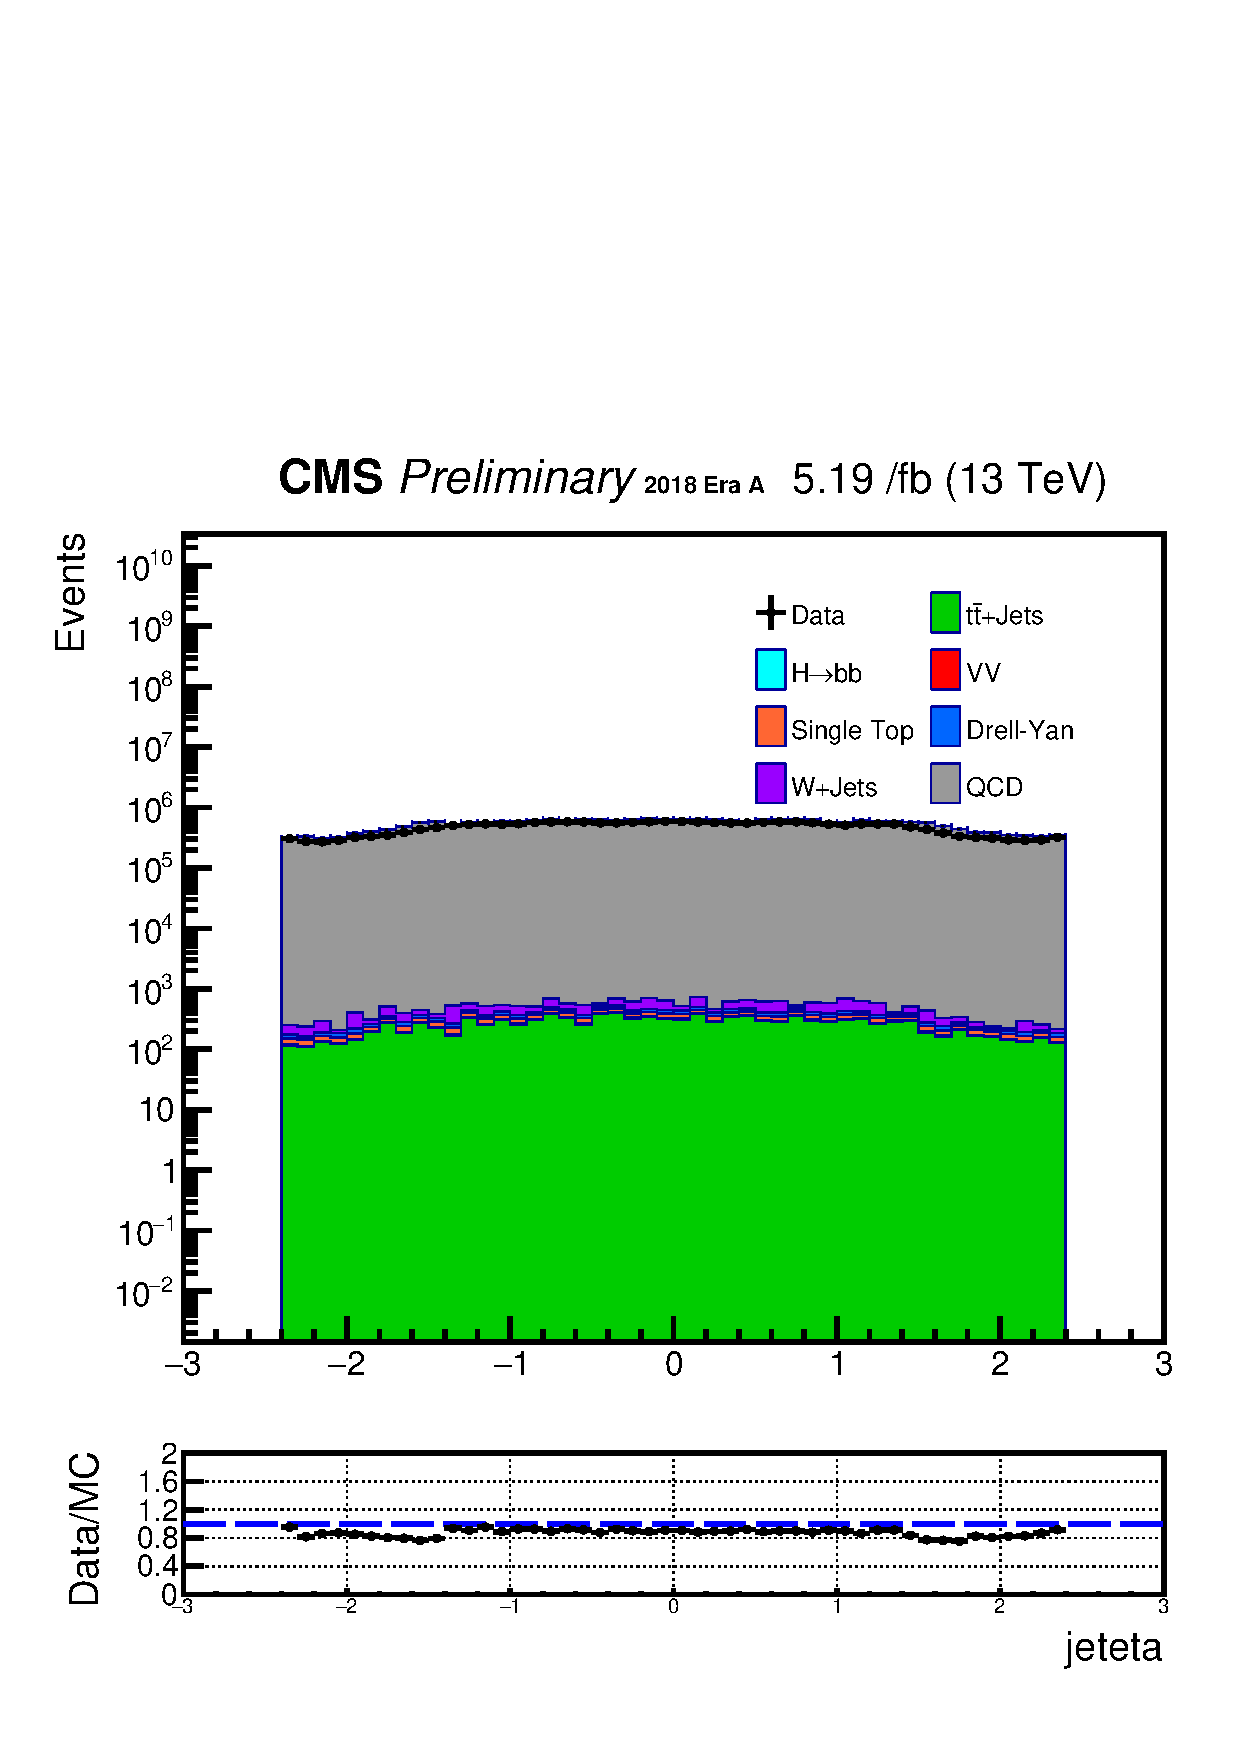
\includegraphics[width=0.47\linewidth]{figs/Data_log_AnalysisNote_MS-15_ctauS-10_jeteta.pdf}
  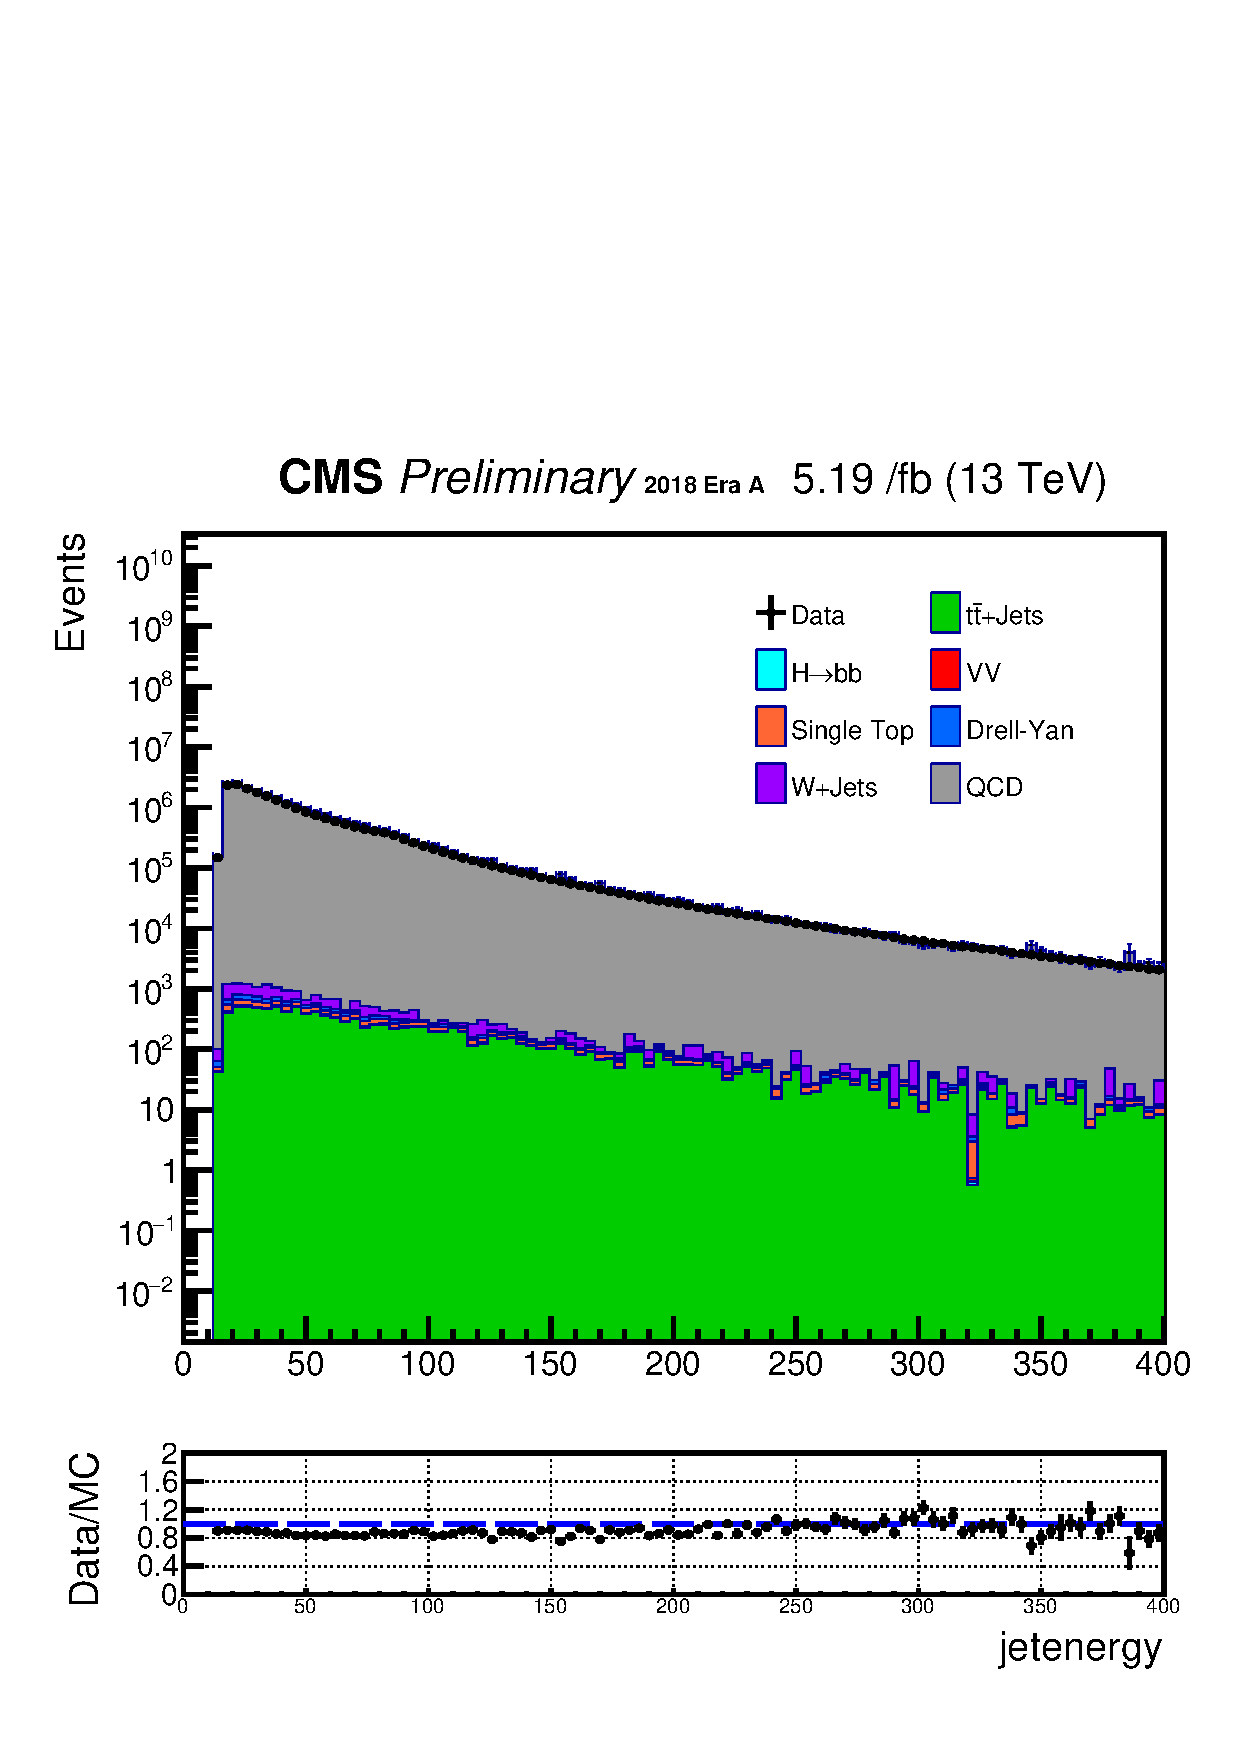
\includegraphics[width=0.47\linewidth]{figs/Data_log_AnalysisNote_MS-15_ctauS-10_jetenergy.pdf}
  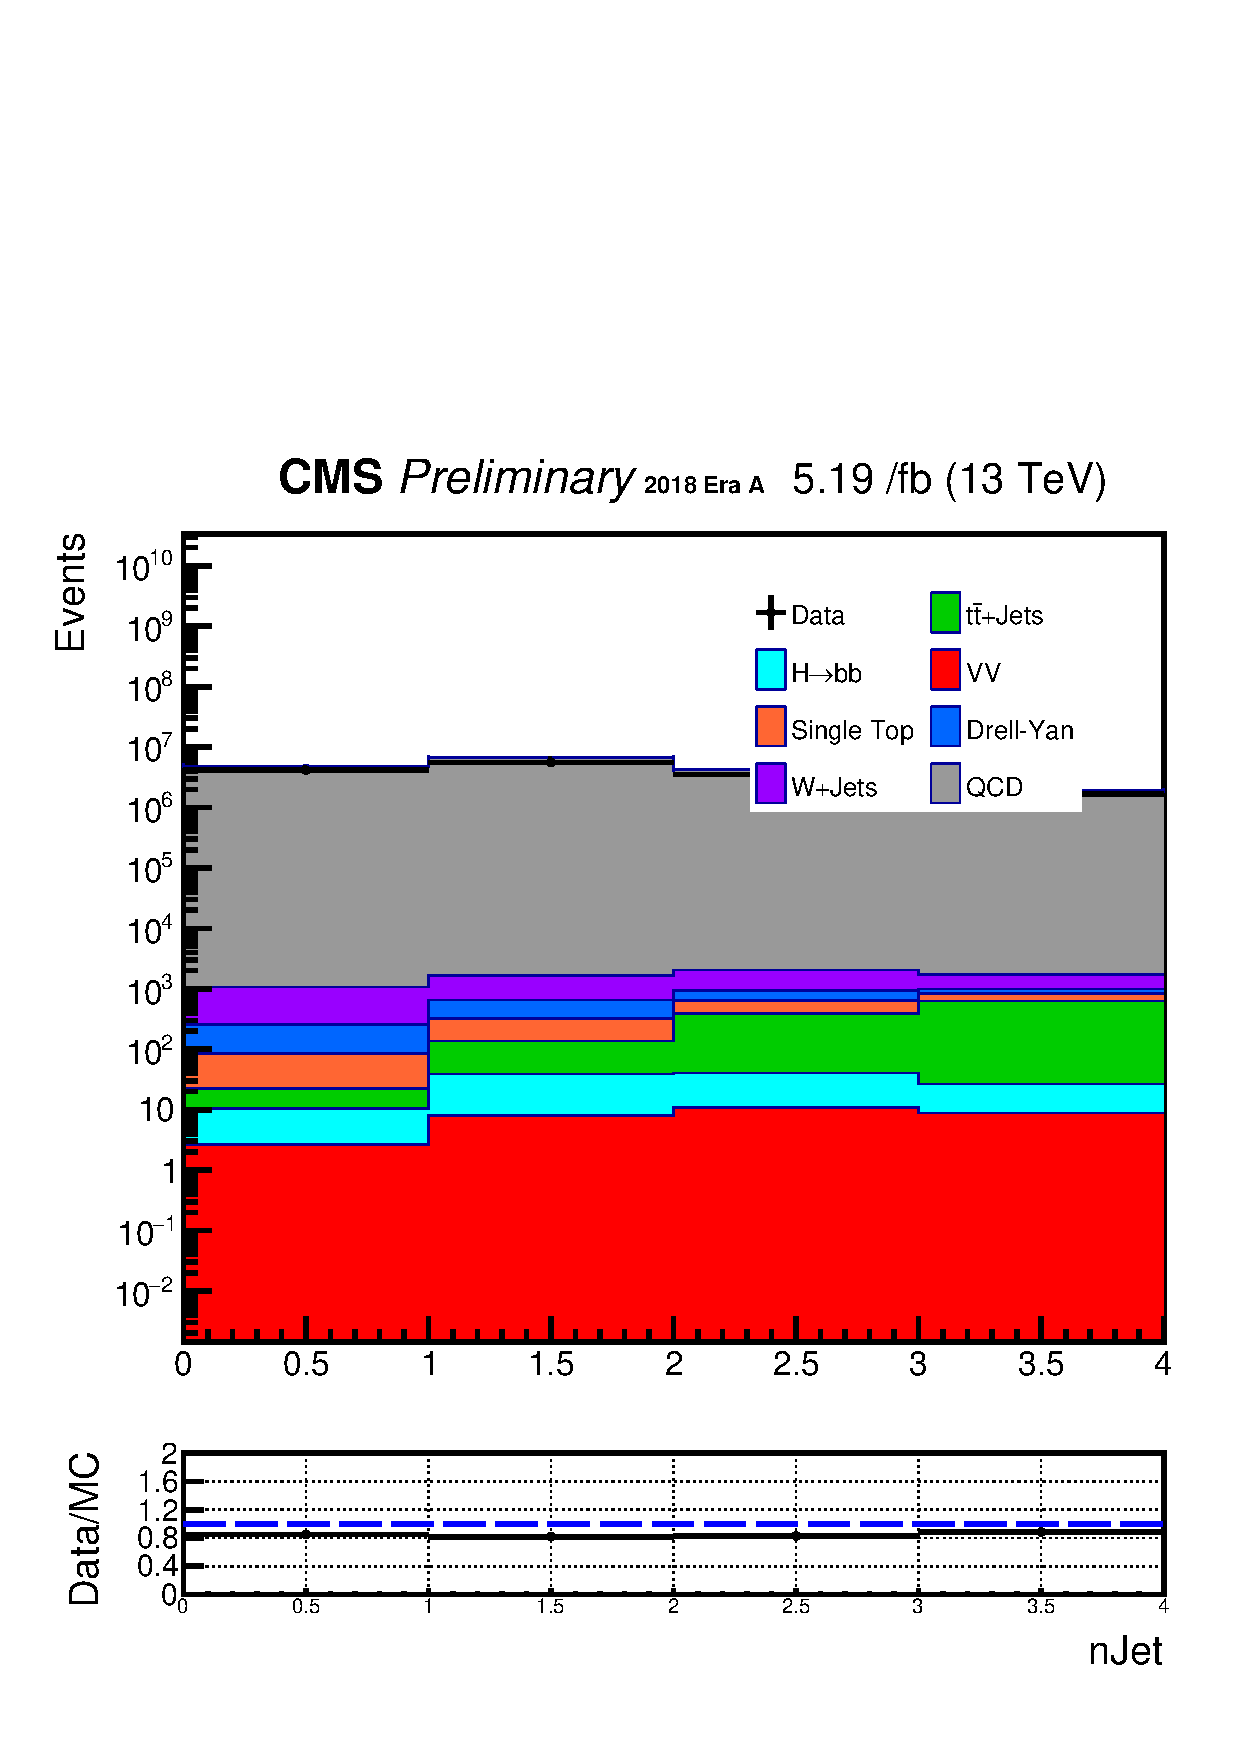
\includegraphics[width=0.47\linewidth]{figs/Data_log_AnalysisNote_MS-15_ctauS-10_nJet.pdf}
\end{figure}

\section{Taus}\label{sec:taus}
Although we do not use $\tau$ leptons for event selection or background estimation, we still plotted essential variables of $\tau$ leptons for review.
The analysis sources ``PAT::slimmedTaus'' from MINIAOD for MC and ``RECO::slimmedTaus'' for Data to produce {\tt selectedTaus}.
$\tau$'s hadronic decay can be reconstructed with PFJets' charged hadrons in HCAL, and 2 $\gamma$s from $\pi^{0}$ decays in ECAL.
$\tau$ objects require
\begin{itemize}
  \item \pt$\geq$ 20\GeV
  \item $|\eta|$ $\leq$ 2.4
\end{itemize}

\begin{figure}[h!]
  \caption{Data/MC of $\tau$ objects for \pt, $\eta$, energy, nJet}
  \label{fig:taus}
  \centering
  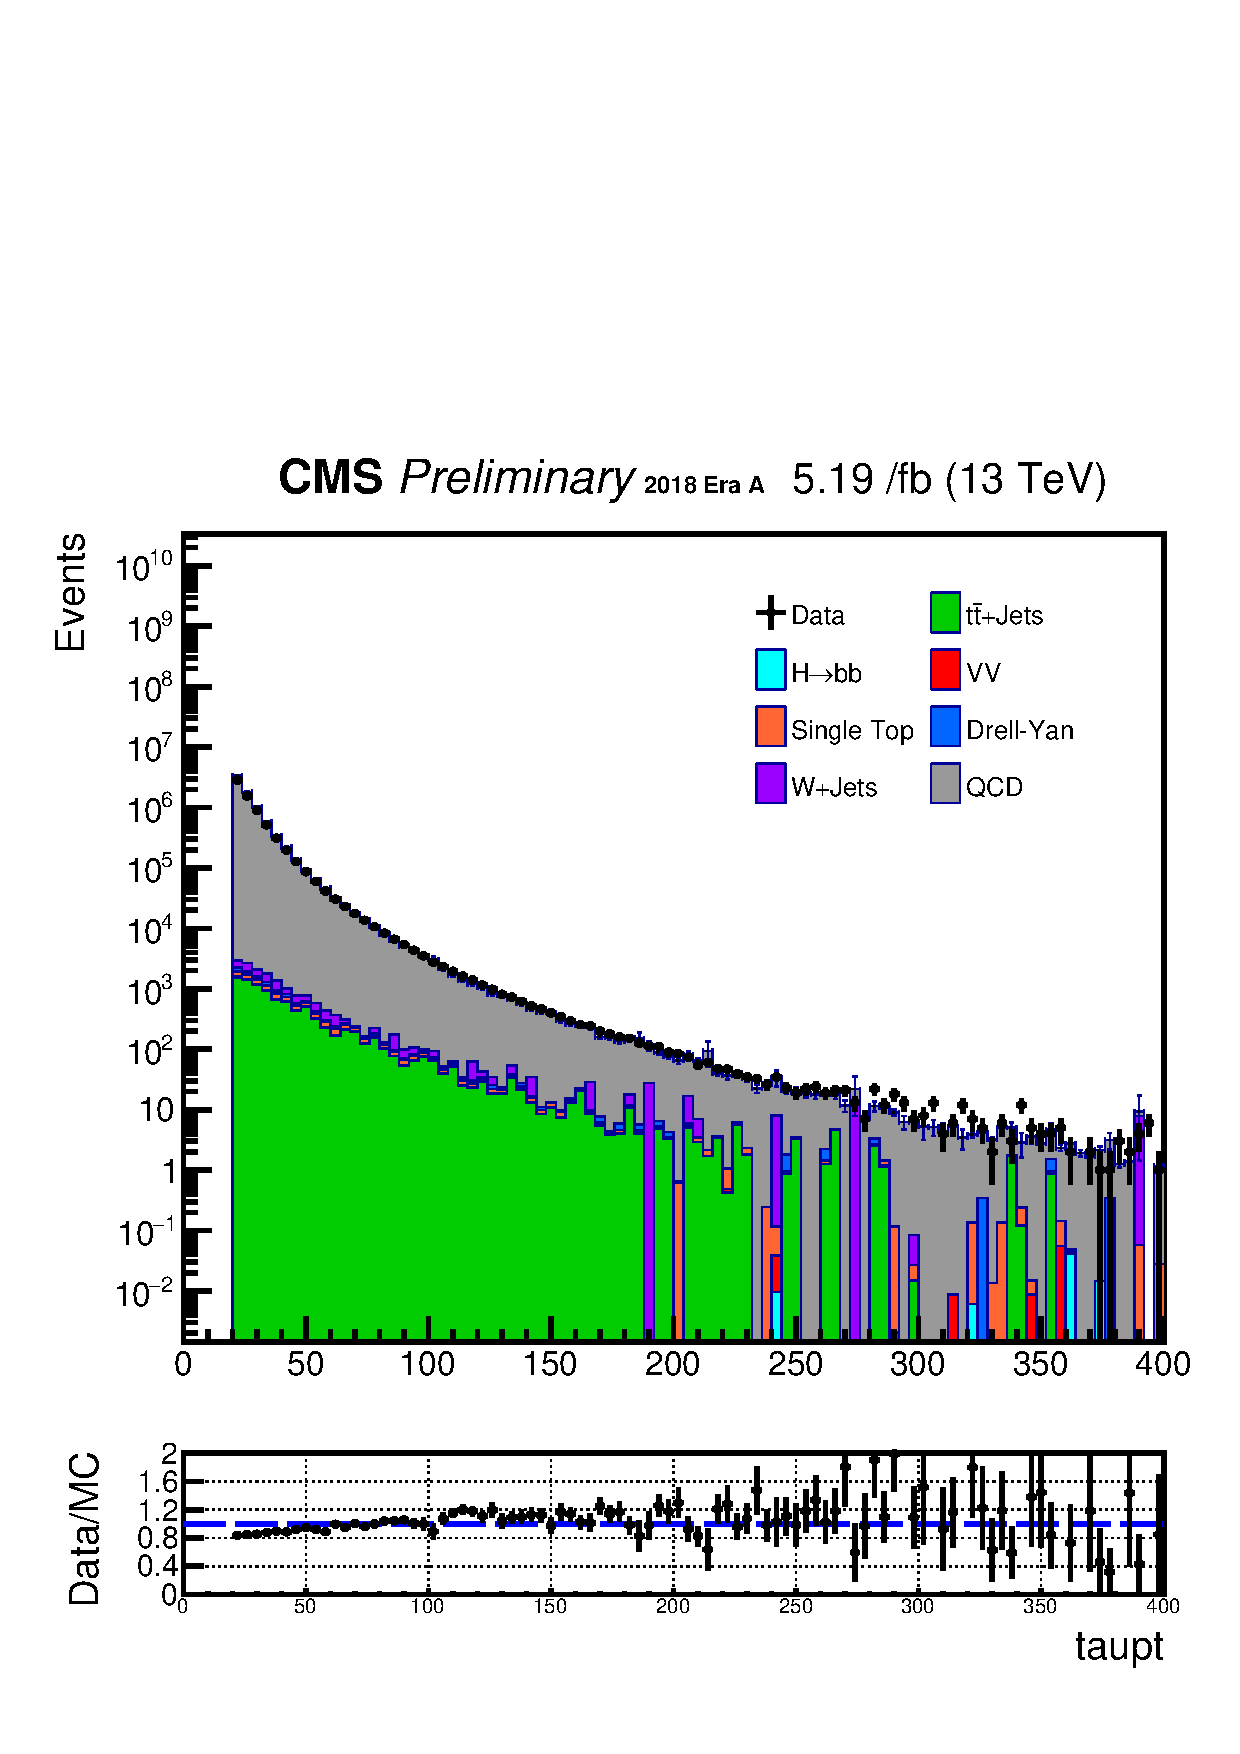
\includegraphics[width=0.47\linewidth]{figs/Data_log_AnalysisNote_MS-15_ctauS-10_taupt.pdf}
  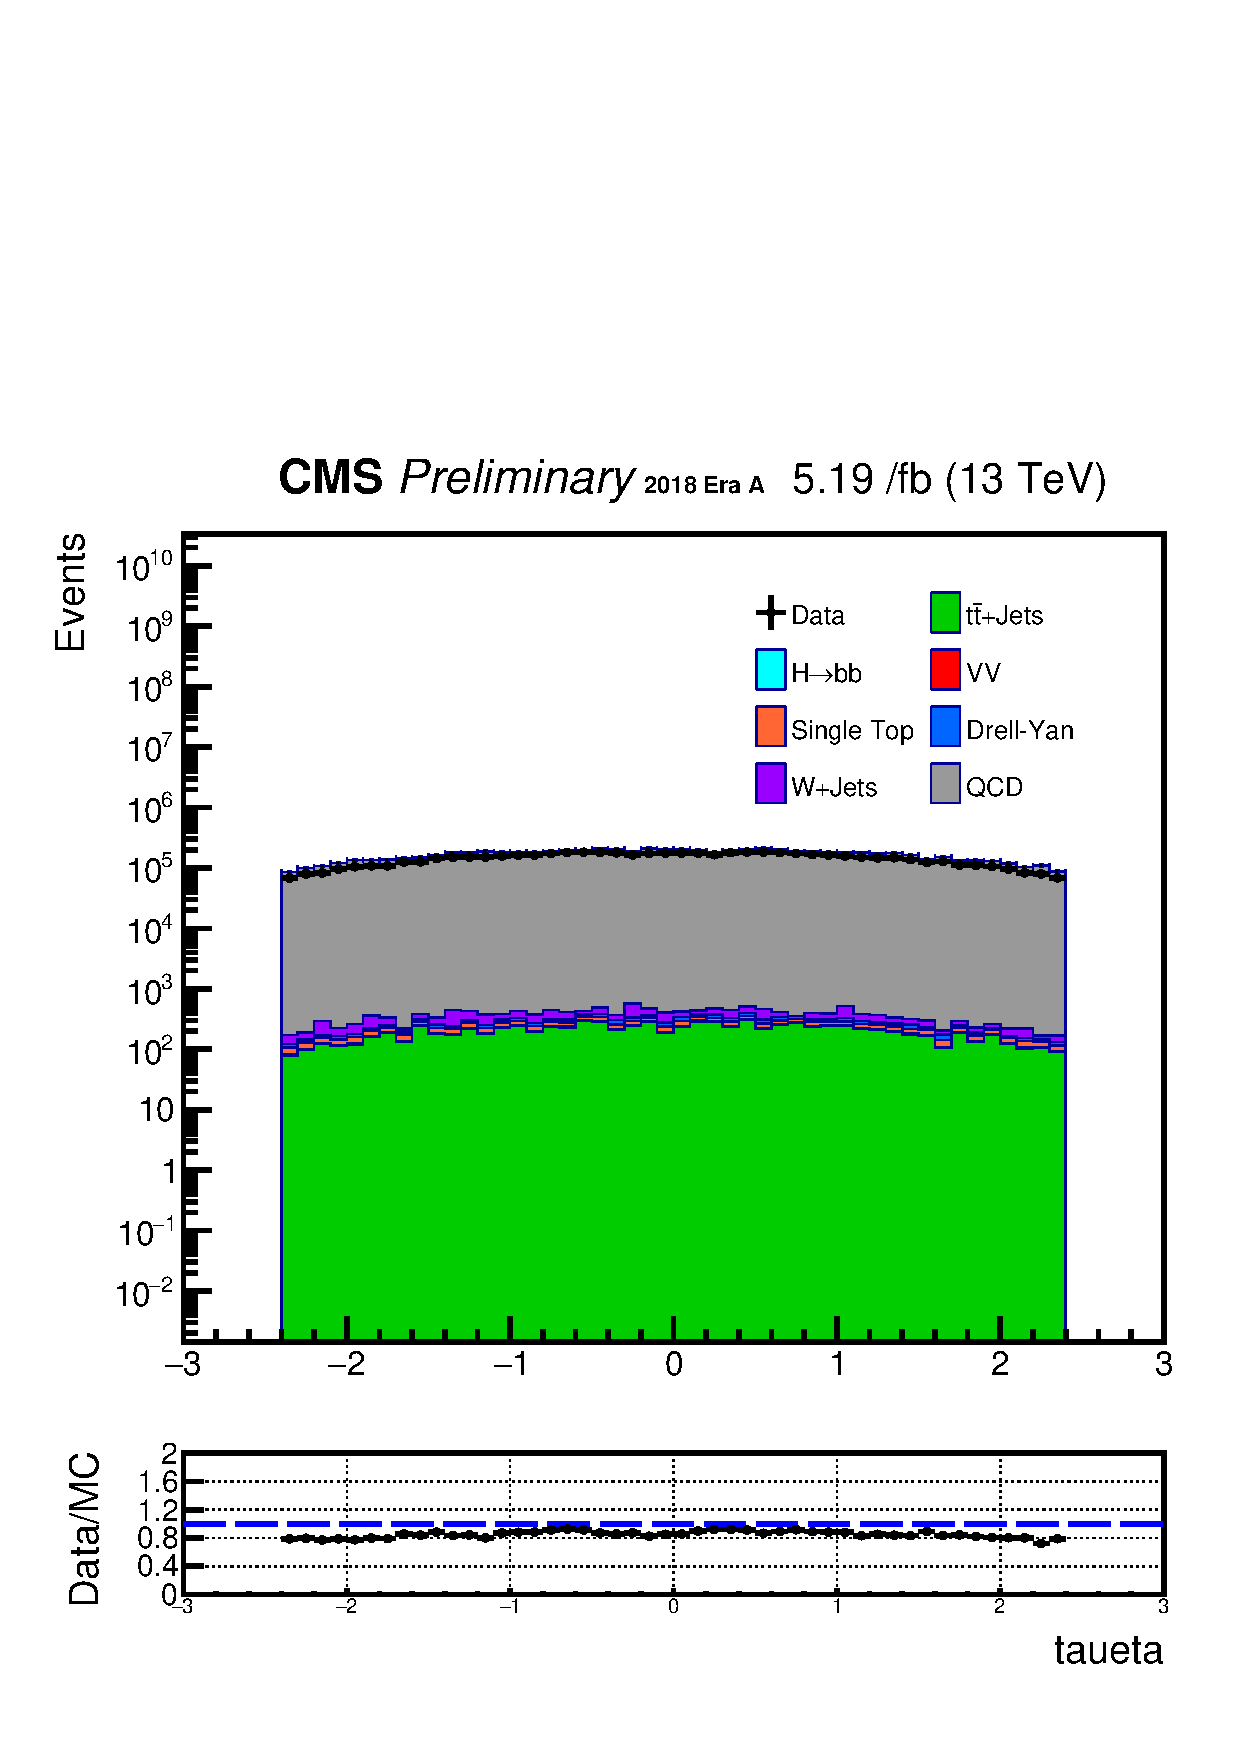
\includegraphics[width=0.47\linewidth]{figs/Data_log_AnalysisNote_MS-15_ctauS-10_taueta.pdf}
  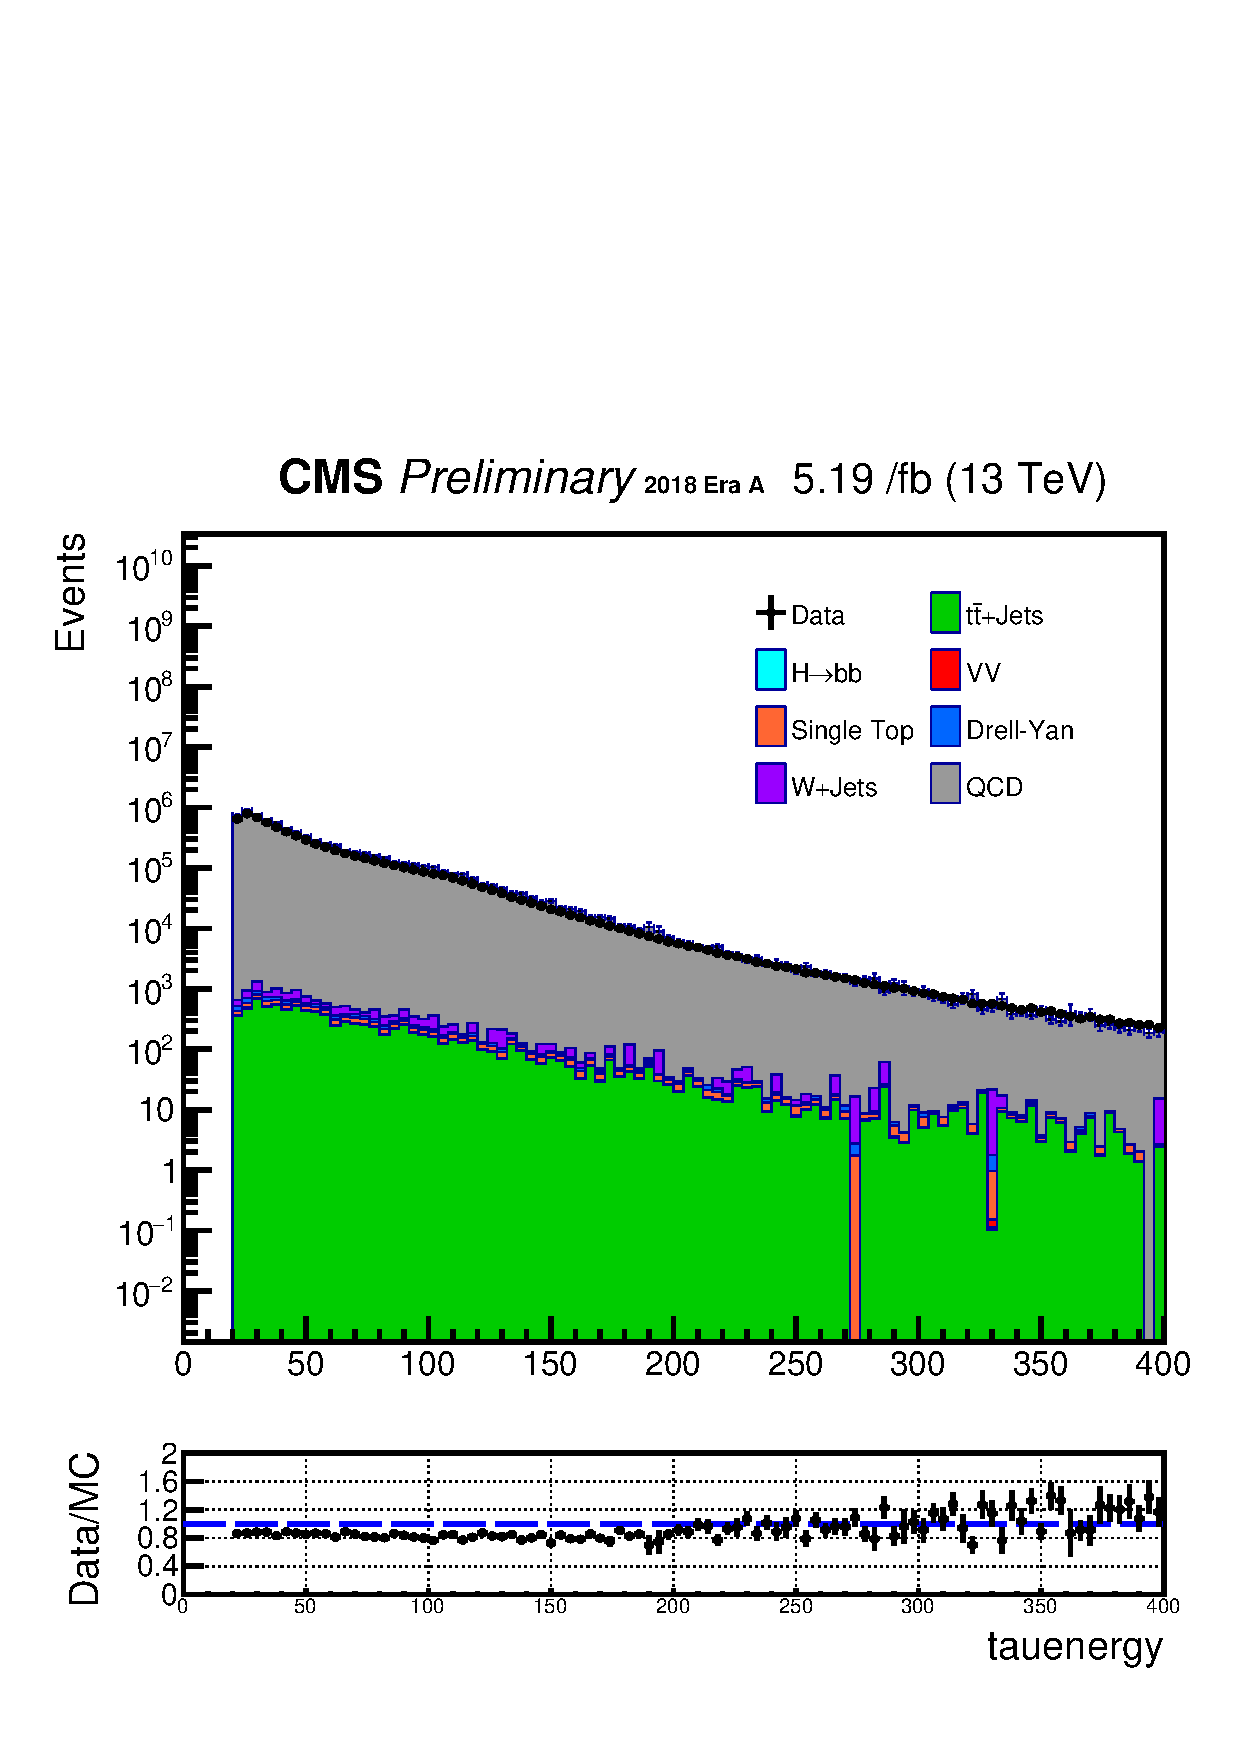
\includegraphics[width=0.47\linewidth]{figs/Data_log_AnalysisNote_MS-15_ctauS-10_tauenergy.pdf}
  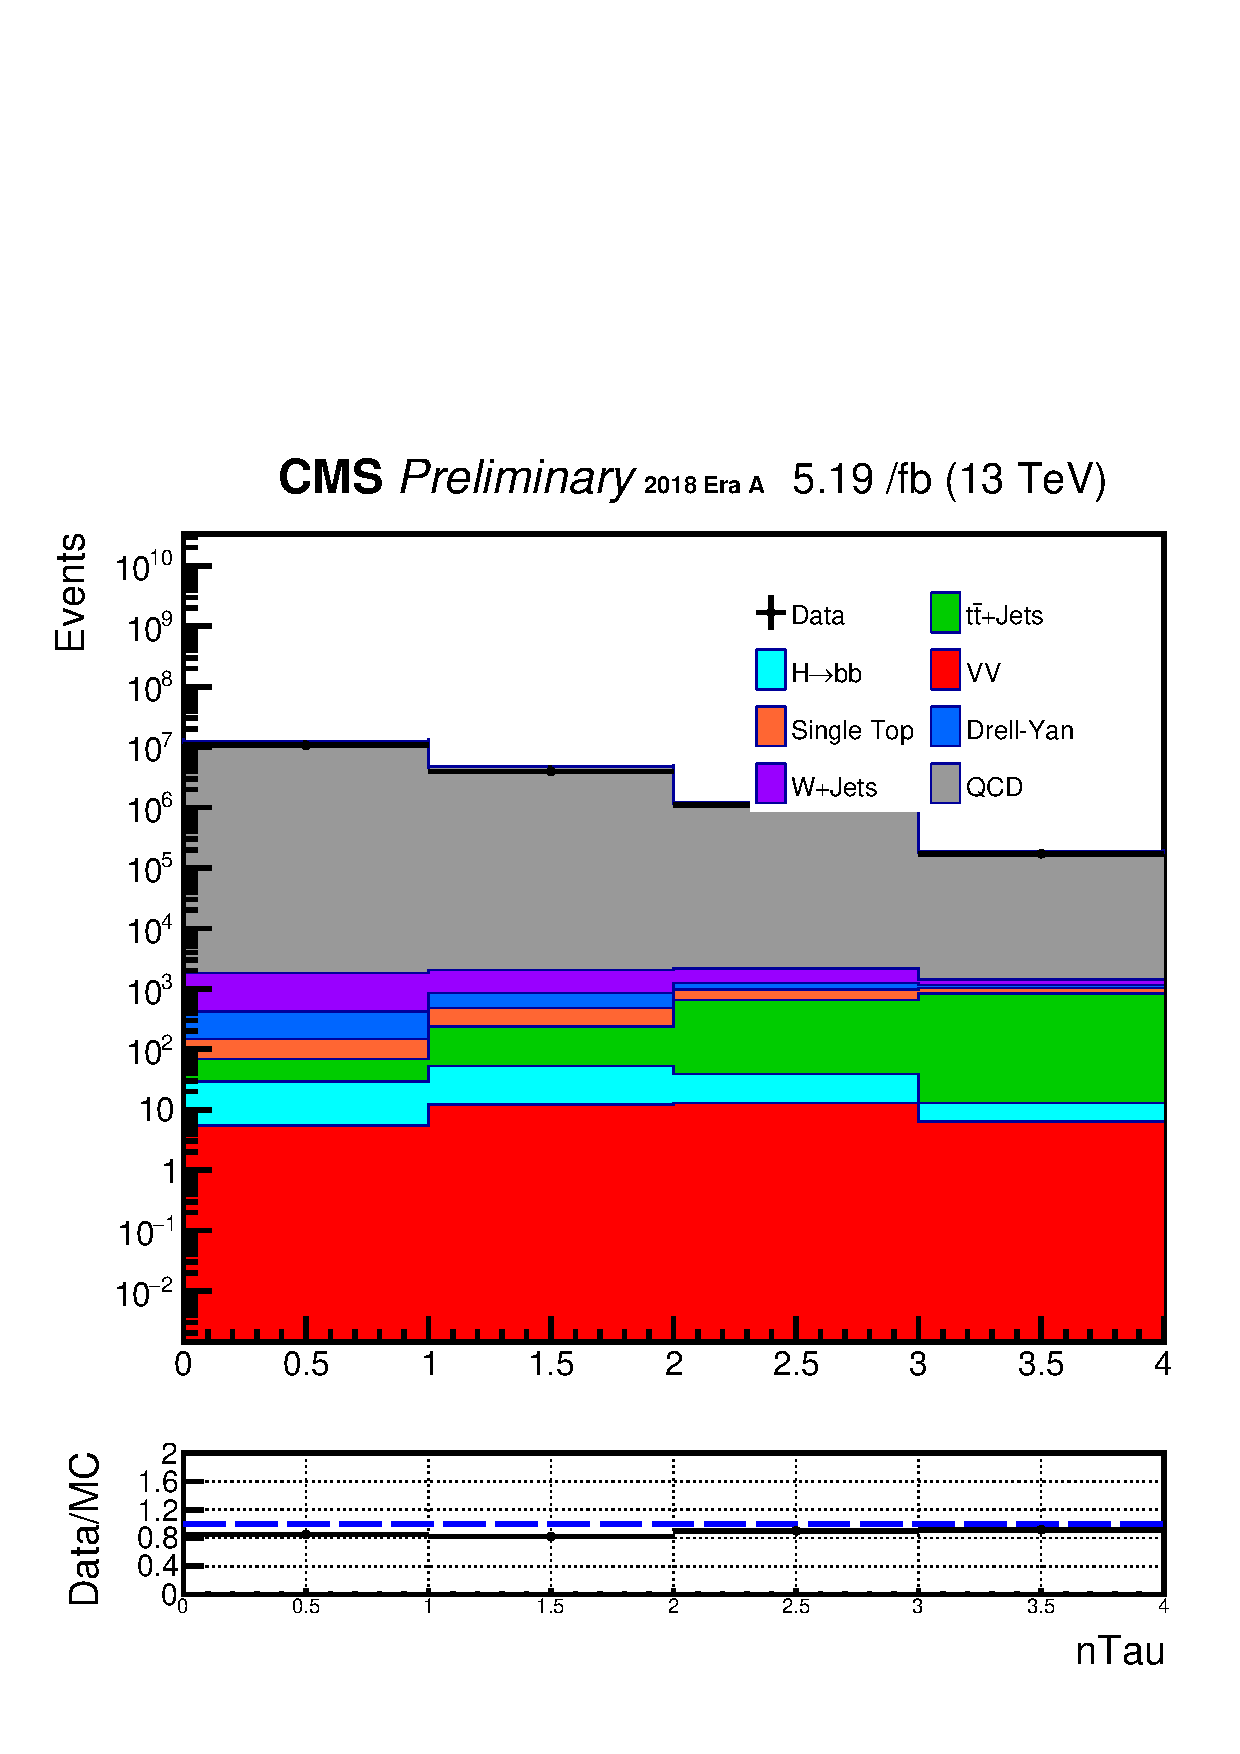
\includegraphics[width=0.47\linewidth]{figs/Data_log_AnalysisNote_MS-15_ctauS-10_nTau.pdf}
\end{figure}

\begin{figure}[h!]
  \caption{Data/MC of MET objects for \pt, energy}
  \label{fig:METs}
  \centering
  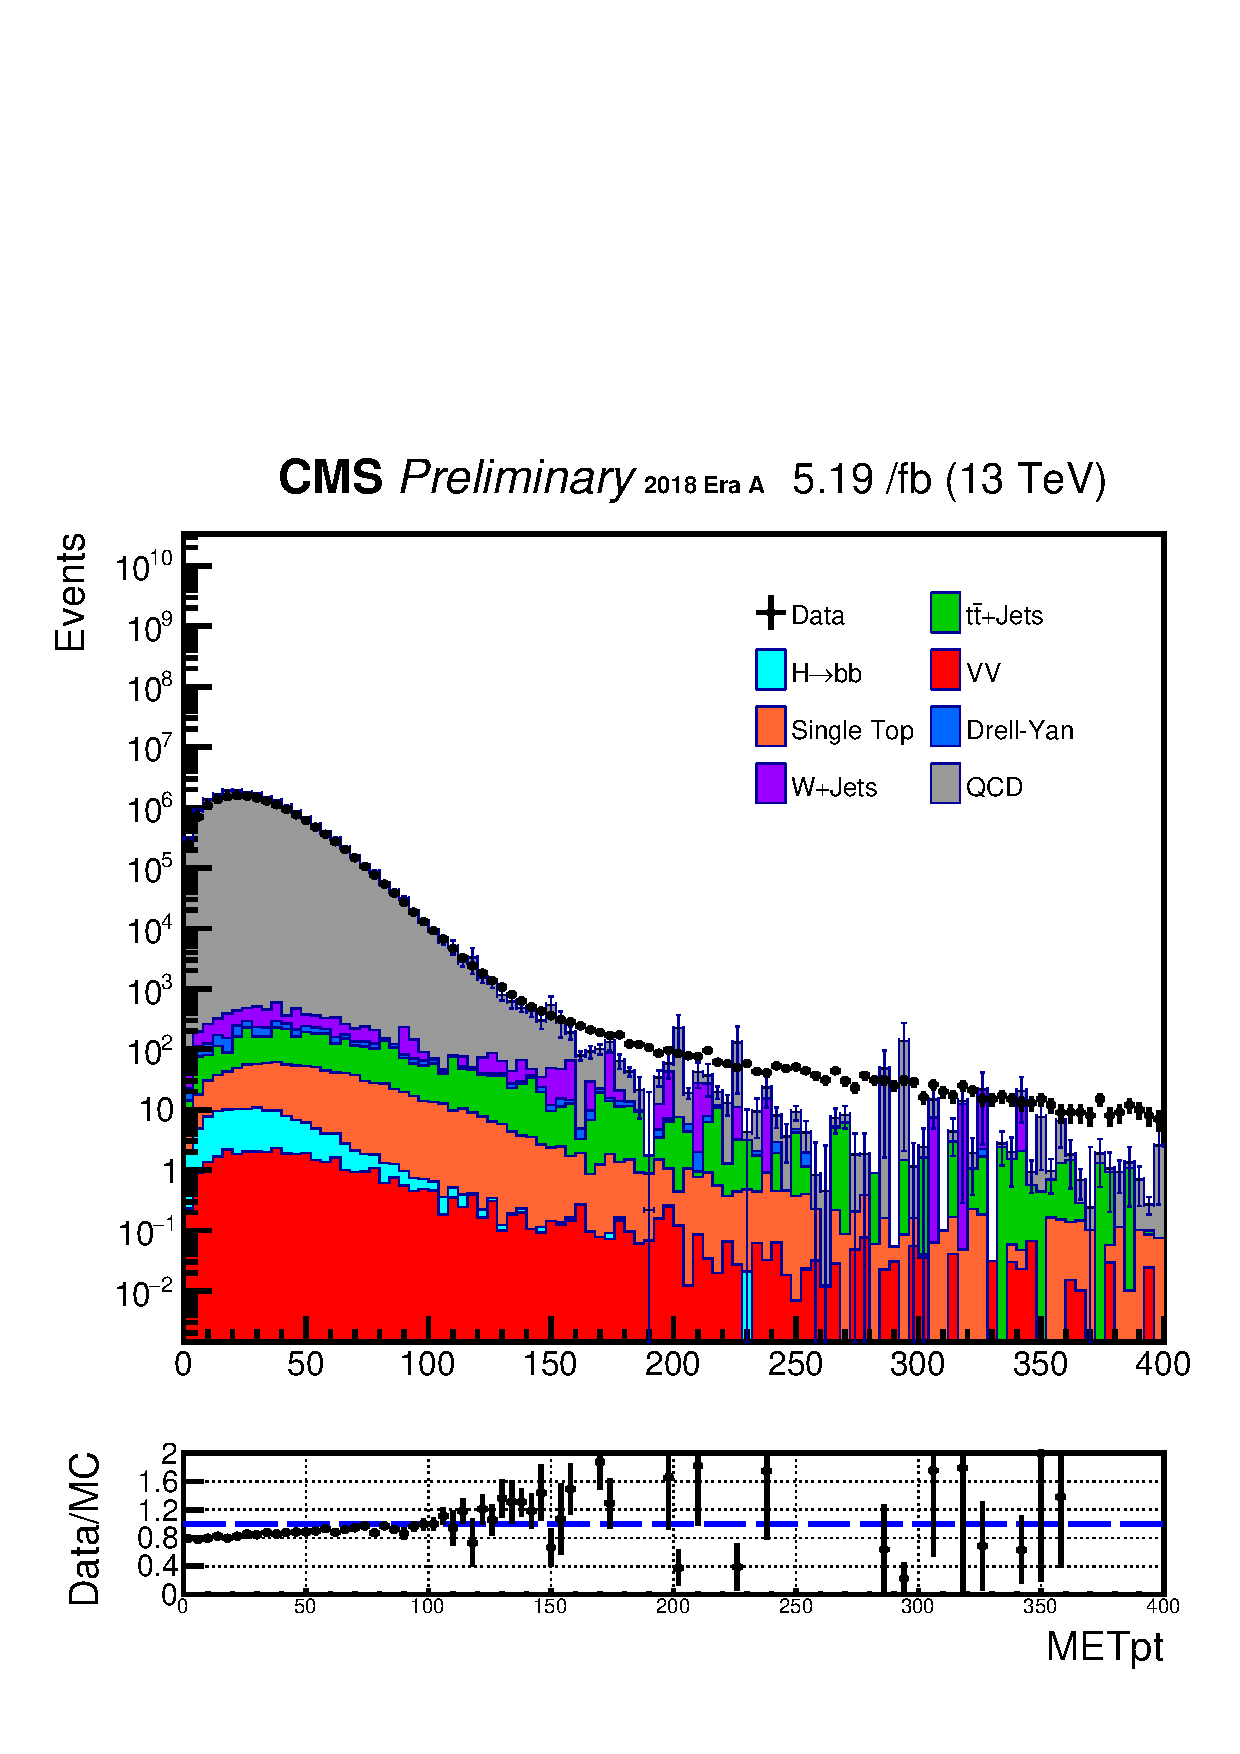
\includegraphics[width=0.47\linewidth]{figs/Data_log_AnalysisNote_MS-15_ctauS-10_METpt.pdf}
  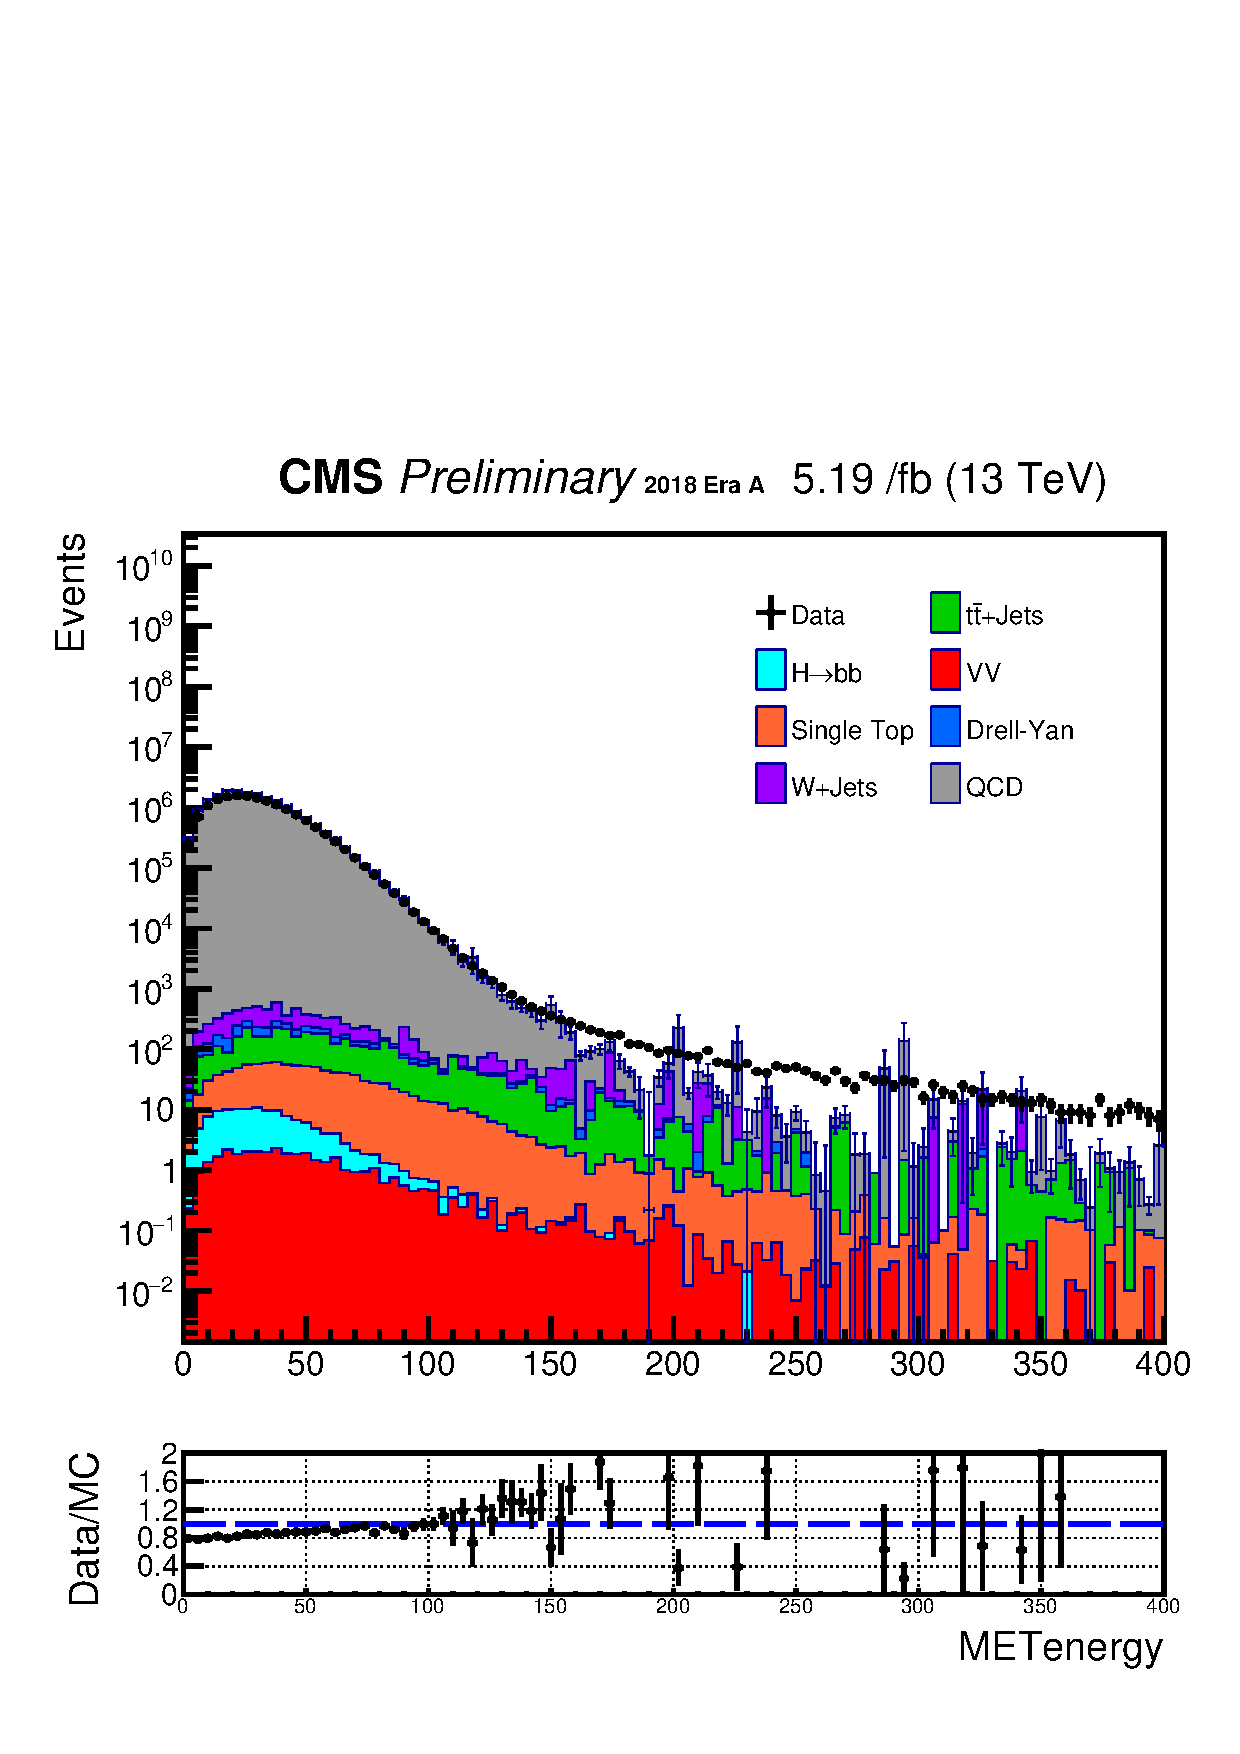
\includegraphics[width=0.47\linewidth]{figs/Data_log_AnalysisNote_MS-15_ctauS-10_METenergy.pdf}
\end{figure}




\section{Region of Interest}\label{sec:ROIs}
Tracks contain many essential qualities, such as the impact parameter significance and the four-vectors.
LLPs decay in the tracker, so these track qualities should be good discriminant against the background.
However, we can not save all tracks in the event with all track information, as much as we have to filter out uninteresting events with the trigger and Data Acquisition system in CMS.
In our signal process, a geometrical concept can play a vital role in sorting out only relevant tracks for our analysis.
LLP has no electric or color charge as described in section \ref{sec:theory}.
LLP leaves no tracks in the tracker and decays into 2 charged $\tau$ leptons, which decay into at least one charged track (muon, electron, at least one charged hadron).
Like in the pair production, two charged tracks often travel opposite directions.
Thus, a geometric convergence of 2 charged tracks should point to the decay vertex of the neutral LLP.
The tracker algorithm we use to construct this ``Interesting Geometric Region'' provides us a converged vertex.
The area around this vertex is referred to as the ``Region of Interest'' (ROI).
The complete reconstruction procedure of the Regions of Interest is detailed in the following subsections.
An ROI requires
\begin{itemize}
  \item Good quality track selection
  \item Vertex Fitted from pair-wise tracks by V0Fitter in CMSSW
  \item Clustering the fitted vertices to form a Region of Intrest (ROI)
  \item Looking for tracks around $\Delta R=0.3$ around ROI to save its isolation information
\end{itemize}

\subsection{Tracks}\label{sec:ROI_tracks}

The analysis sources ``packedPFCandidates'' and ``lostTracks'' from MINIAOD.
Track parameters and convariance values will be propagated along the ROI production process and no value should be non-physical
\begin{itemize}
  \item !isinf(tracks.parameter)  and !isnan(tracks.parameter) 
  \item !isinf(tracks.covariance) and !isnan(tracks.covariance) 
  \item Number of valid hits $>$ 3
  \item \pt $\geq$ 0.35
  \item Track $IPSig_{XY}\geq$2.
  \item Track $IPSig_{Z}\geq$-1.
  \item Track normalized $\chi^{2}\geq$10.
\end{itemize}


\subsection{Vertex Fitter}\label{sec:ROI_V0Fitter}

The analysis sources ``offlineBeamspot'' from MINIAOD for beamspot reference.
Vertex fitter is ``KalmanVertexFitter'' with vertex cuts as below.
\begin{itemize}
  \item Vertex $\chi^{2}\geq$6.63 
  \item Transverse Decay distance significance$\geq$15.
  \item V0mass $\geq$13000\GeV
  \item cos($\theta_{XY}$) between x and p of V0 candidate $\geq$ 0
  \item cos($\theta_{XYZ}$) between x and p of V0 candidate $\geq$ -2
\end{itemize}
%New PVtight and opposite traveling track req

\subsection{ROI formation}\label{sec:ROI_ROIformation}
Fitted vertices are clustered to form a Region of Interest (ROI).
The clustering steps can be further detailed as below.
\begin{itemize}
  \item A fitted vertex is merged with another vertex if they are within 1cm. 
  \item A new ROI is formed where the position vector of ROI is averaged.
  \item Clustering is repeated until there is no other vertex within 1cm limit.
\end{itemize}
Although vertex clustering can be done with the step above, we can be creative and acquire more information.
Isolation, containing information about the ROI's environment, could also be helpful information.
We can obtain information about isolation by defining an isolation shell.
The shell's construction step is described below.
\begin{itemize}
  \item A cone of DeltaR $\leq$ 0.3 around the center of the ROI is defined, where DeltaR is calculated with respect to the PV.
  \item A plane that is perpendicular to the axis of the cone and that contains the center of the ROI is the isolation plane. It becomes a circle. 
  \item Make the circle into a 3D sphere.
  \item Any tracks that pass through that sphere but not through the ROI are the annulus tracks.
\end{itemize}
With these essential tracks' information, we are ready to discriminate signals from the background.

\begin{figure}[h!]
  \centering
  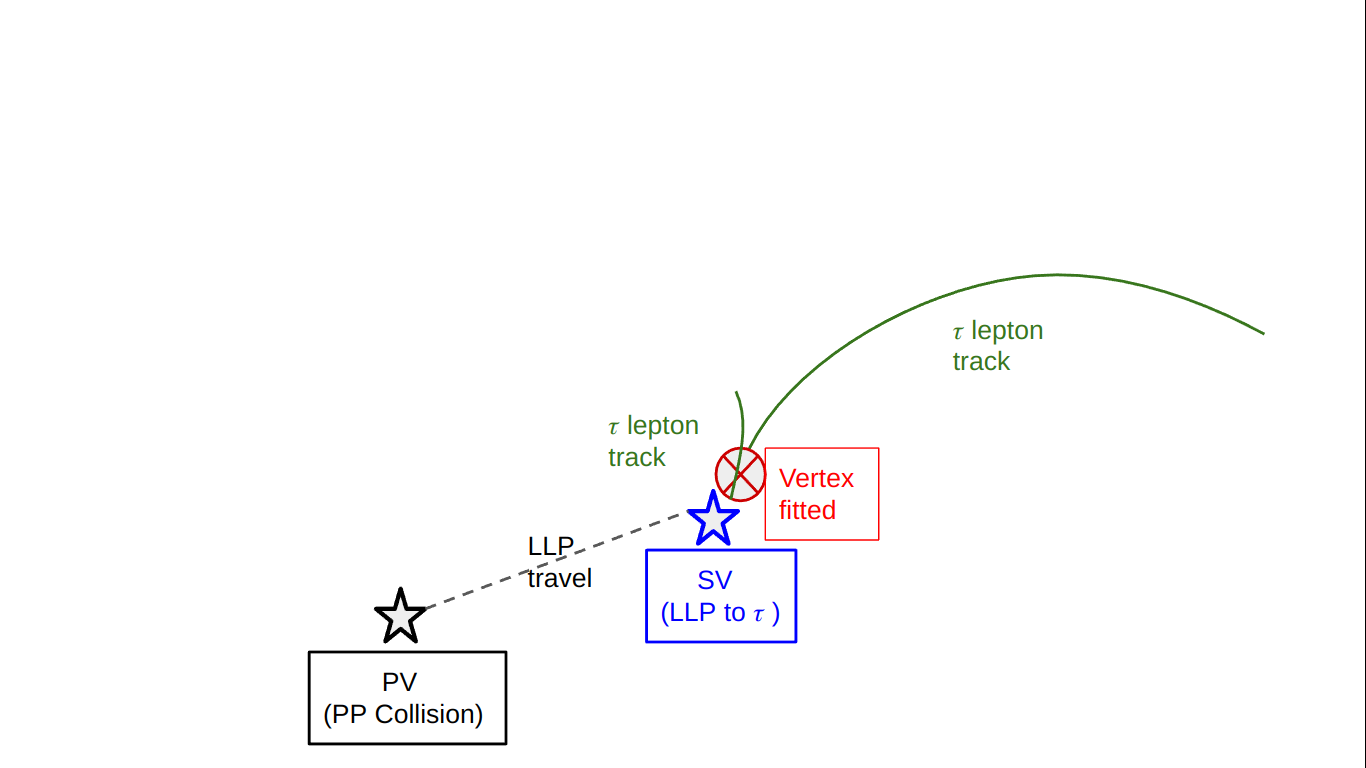
\includegraphics[width=0.65\linewidth]{figs/ROICT1.png}
  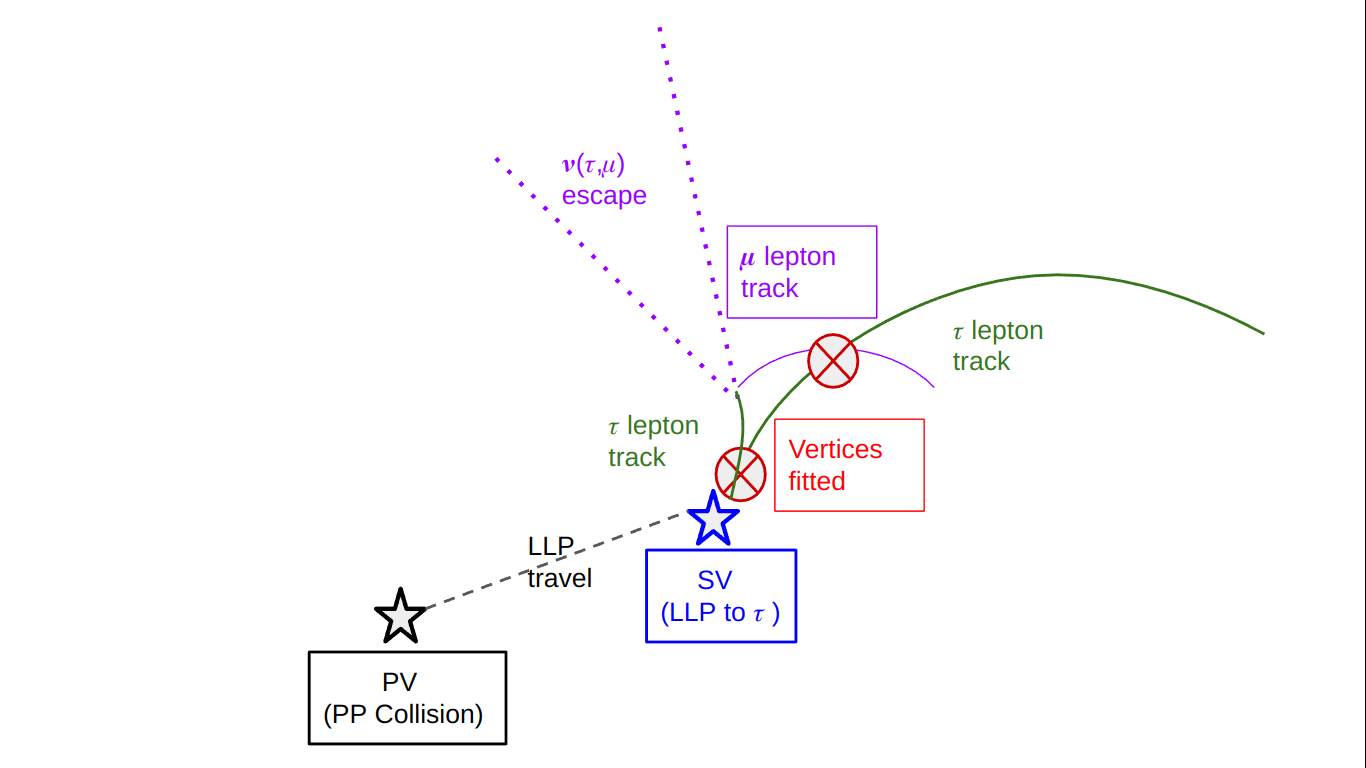
\includegraphics[width=0.65\linewidth]{figs/ROICT2.png}
  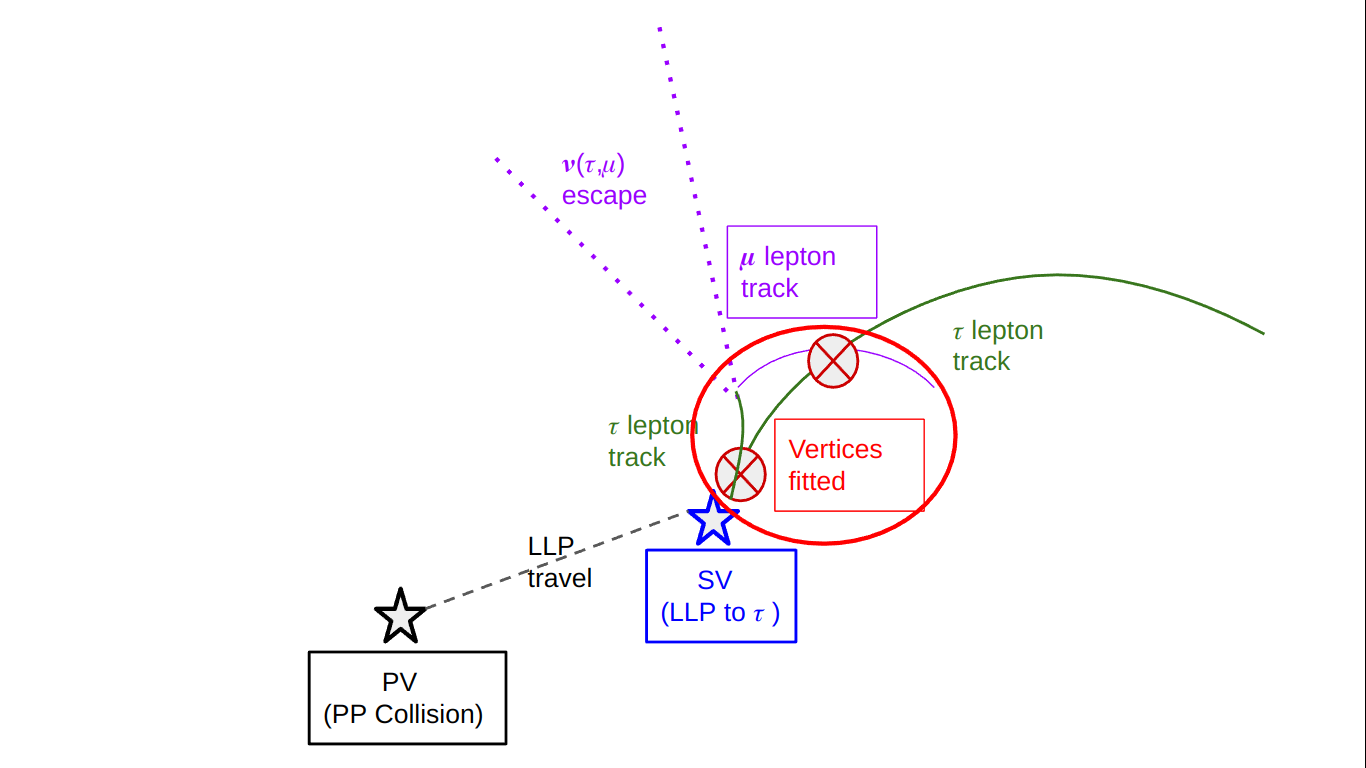
\includegraphics[width=0.65\linewidth]{figs/ROICT3.png}
\caption{
        The figures display cartoons of the step-by-step formation of the Region of Interest (ROI).
	After LLP travels from the Primary Vertex (PV) to Secondary Vertex (SV), it leaves no track, and decays into a tau lepton pair.
	Tau lepton pair's tracks are recorded in the tracker, as denoted in green color lines.
	The first figure shows the vertex (red star) fitted by KalmanVertexFitter in CMSSW from two charged tracks that decayed from a neutral LLP.
        The second figure shows fitting procedure of another vertex. With one of tau leptons decaying into a muon, the muon track crosses the parter tau lepton track and forms a new vertex near the original vertex.
	The third figure shows the clustering of the vertex, with the second vertex formed by the extended tracks being clustered into the original ROI if the vertices are within a 1cm limit.
	}
  \label{fig:Clustering}
\end{figure}

\begin{figure}[h!]
  \centering
  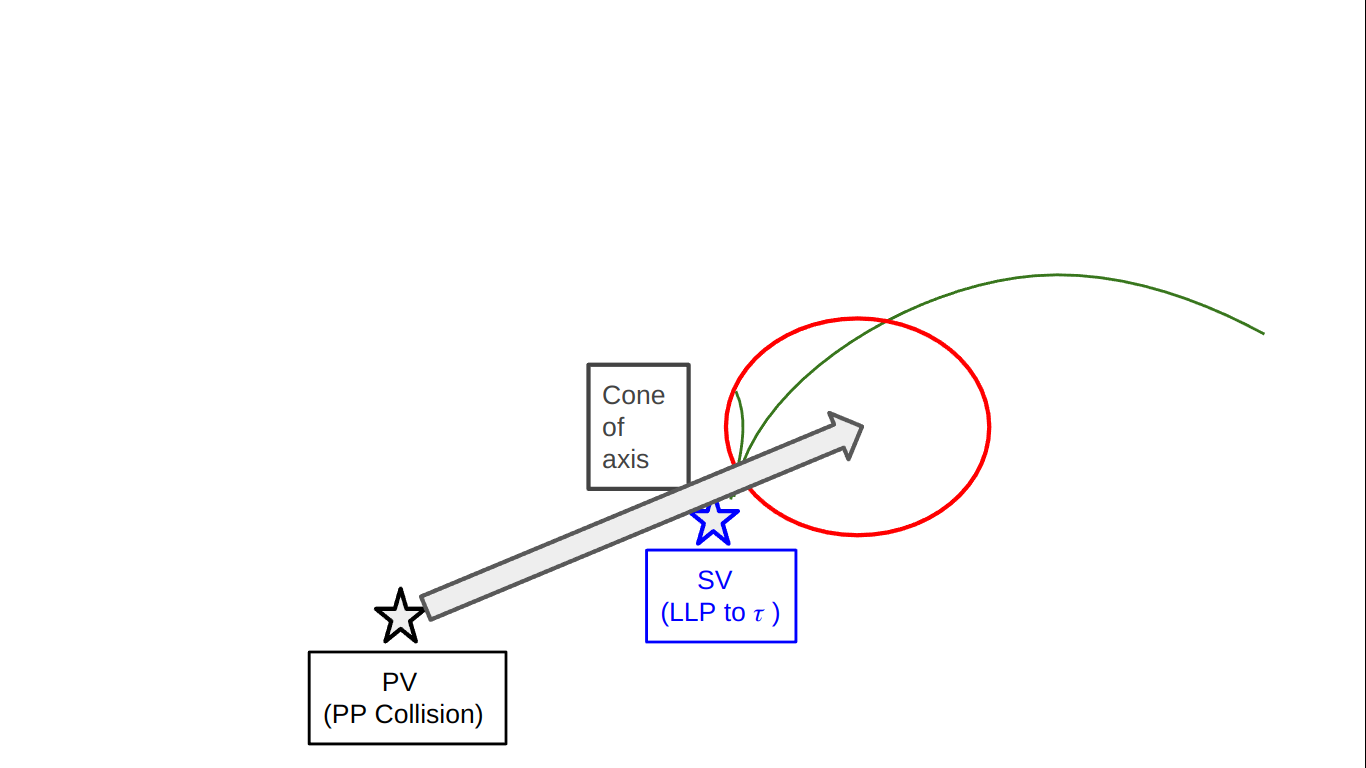
\includegraphics[width=0.65\linewidth]{figs/ROICT4.png}
  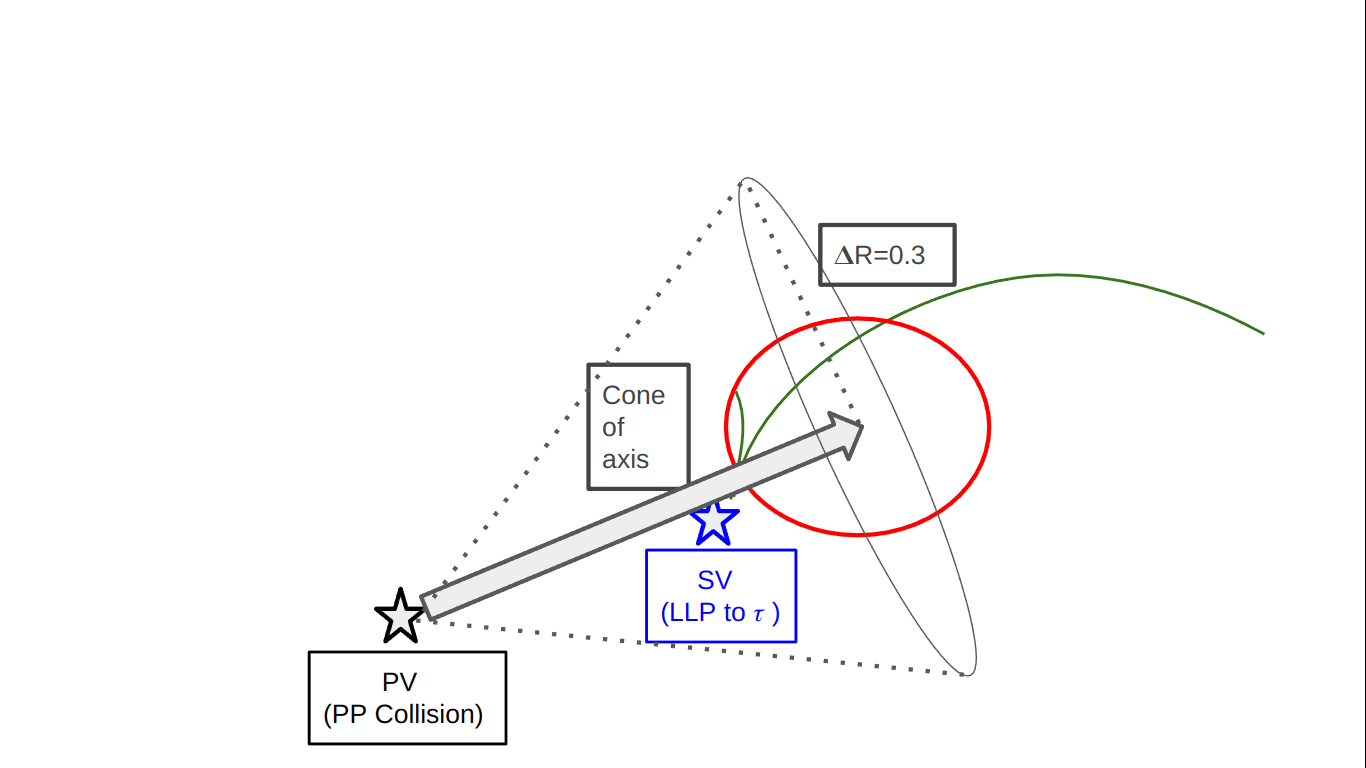
\includegraphics[width=0.65\linewidth]{figs/ROICT5.png}
  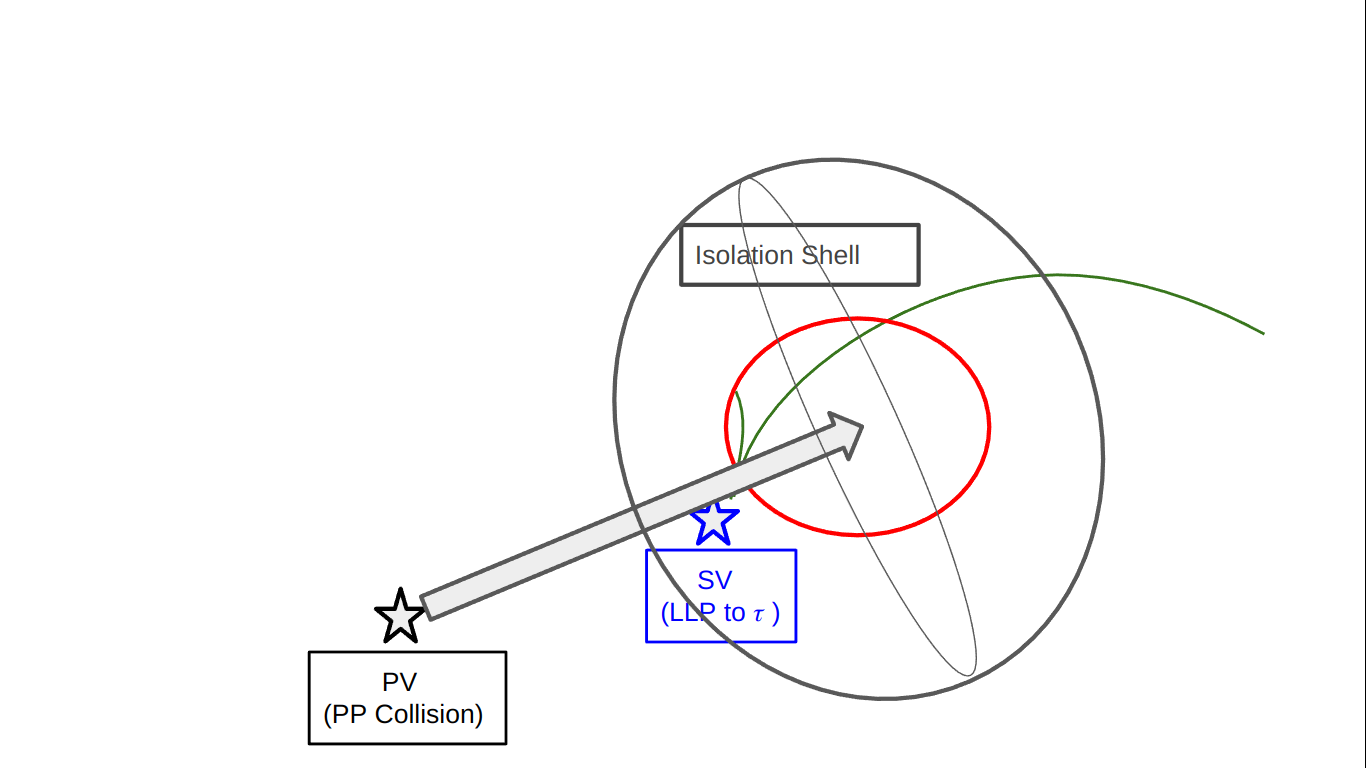
\includegraphics[width=0.65\linewidth]{figs/ROICT6.png}
\caption{
        The figures display cartoons of the step-by-step formation of the shell structure.
        The first figure shows the axis of the cone when the axis goes through the center of ROI.
        The second figure shows the construction of the isolation plane, with $\Delta$ = 0.3 parameter.
        The third figure shows the construction of the isolation shell, with the isolation plane becoming a sphere.
	}
  \label{fig:Clustering2}
\end{figure}

\begin{figure}[h!]
  \centering
  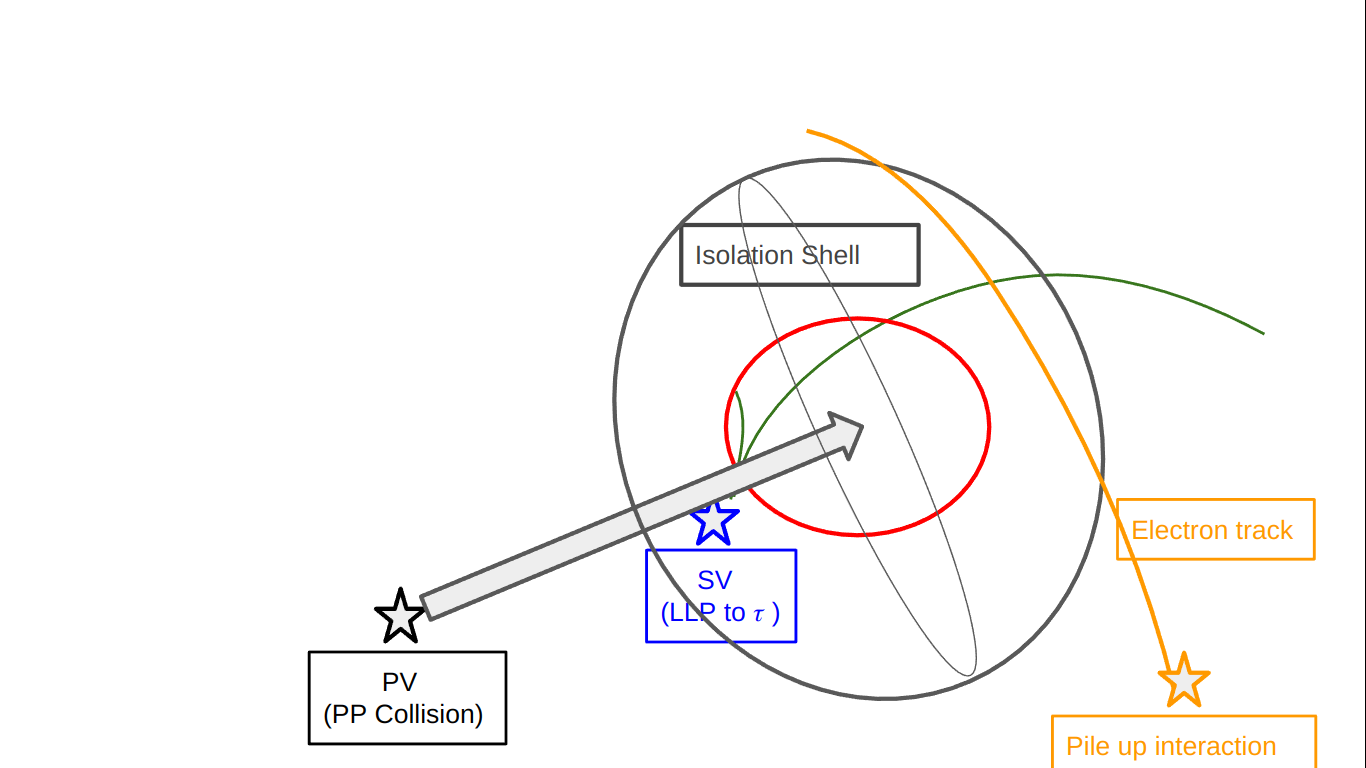
\includegraphics[width=0.7\linewidth]{figs/ROICT7.png}
  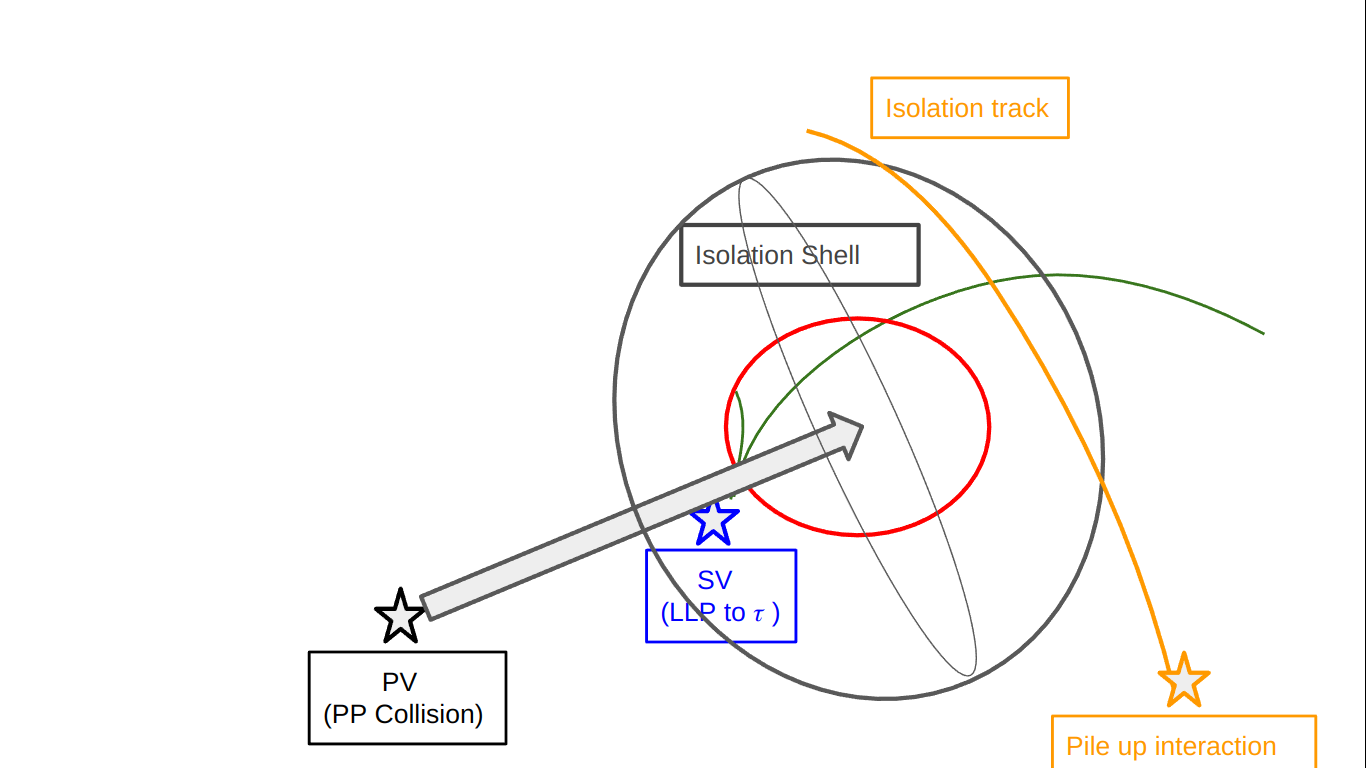
\includegraphics[width=0.7\linewidth]{figs/ROICT8.png}
\caption{
        The figures display cartoons of the step-by-step inclusion of isolation track information.
	The first figure shows an electron or charged hadron track (orange color) originating from a Pile-up interaction.
        One can see the pileup track goes through the isolation shell in the cartoon.
        The second figure shows that the track is outside of the ROI and inside of the isolation shell.
        Thus, the track becomes an isolation track. 
	}
  \label{fig:Clustering3}
\end{figure}


%\begin{figure}[h!]
%	\caption{Data/MC of ROI distribution, distance along the transverse plane (xy plane) and beam direction ($\hat{z}$)}
%  \label{fig:ROIs}
%  \centering
%  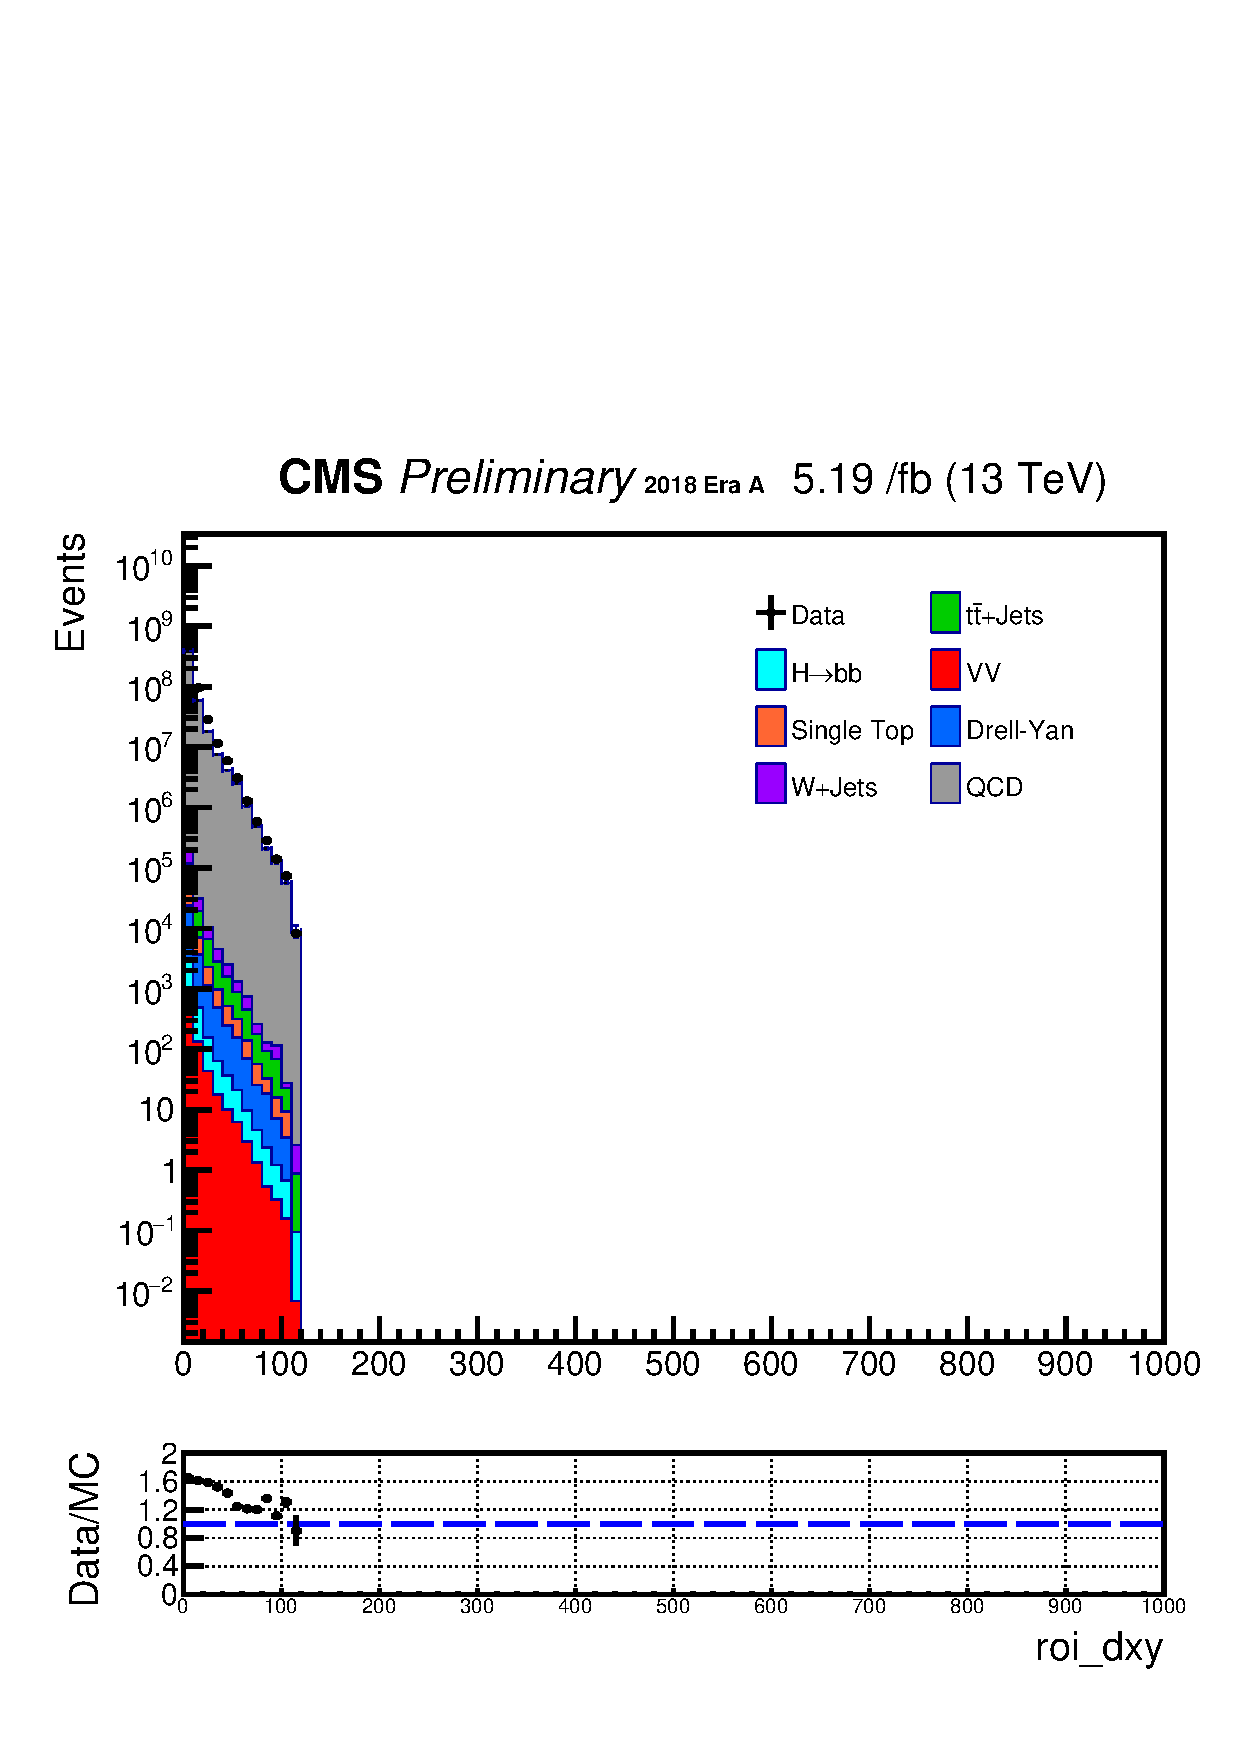
\includegraphics[width=0.47\linewidth]{figs/Data_log_Oct6ANVars_MS-15_ctauS-10_roi_dxy.pdf}
%  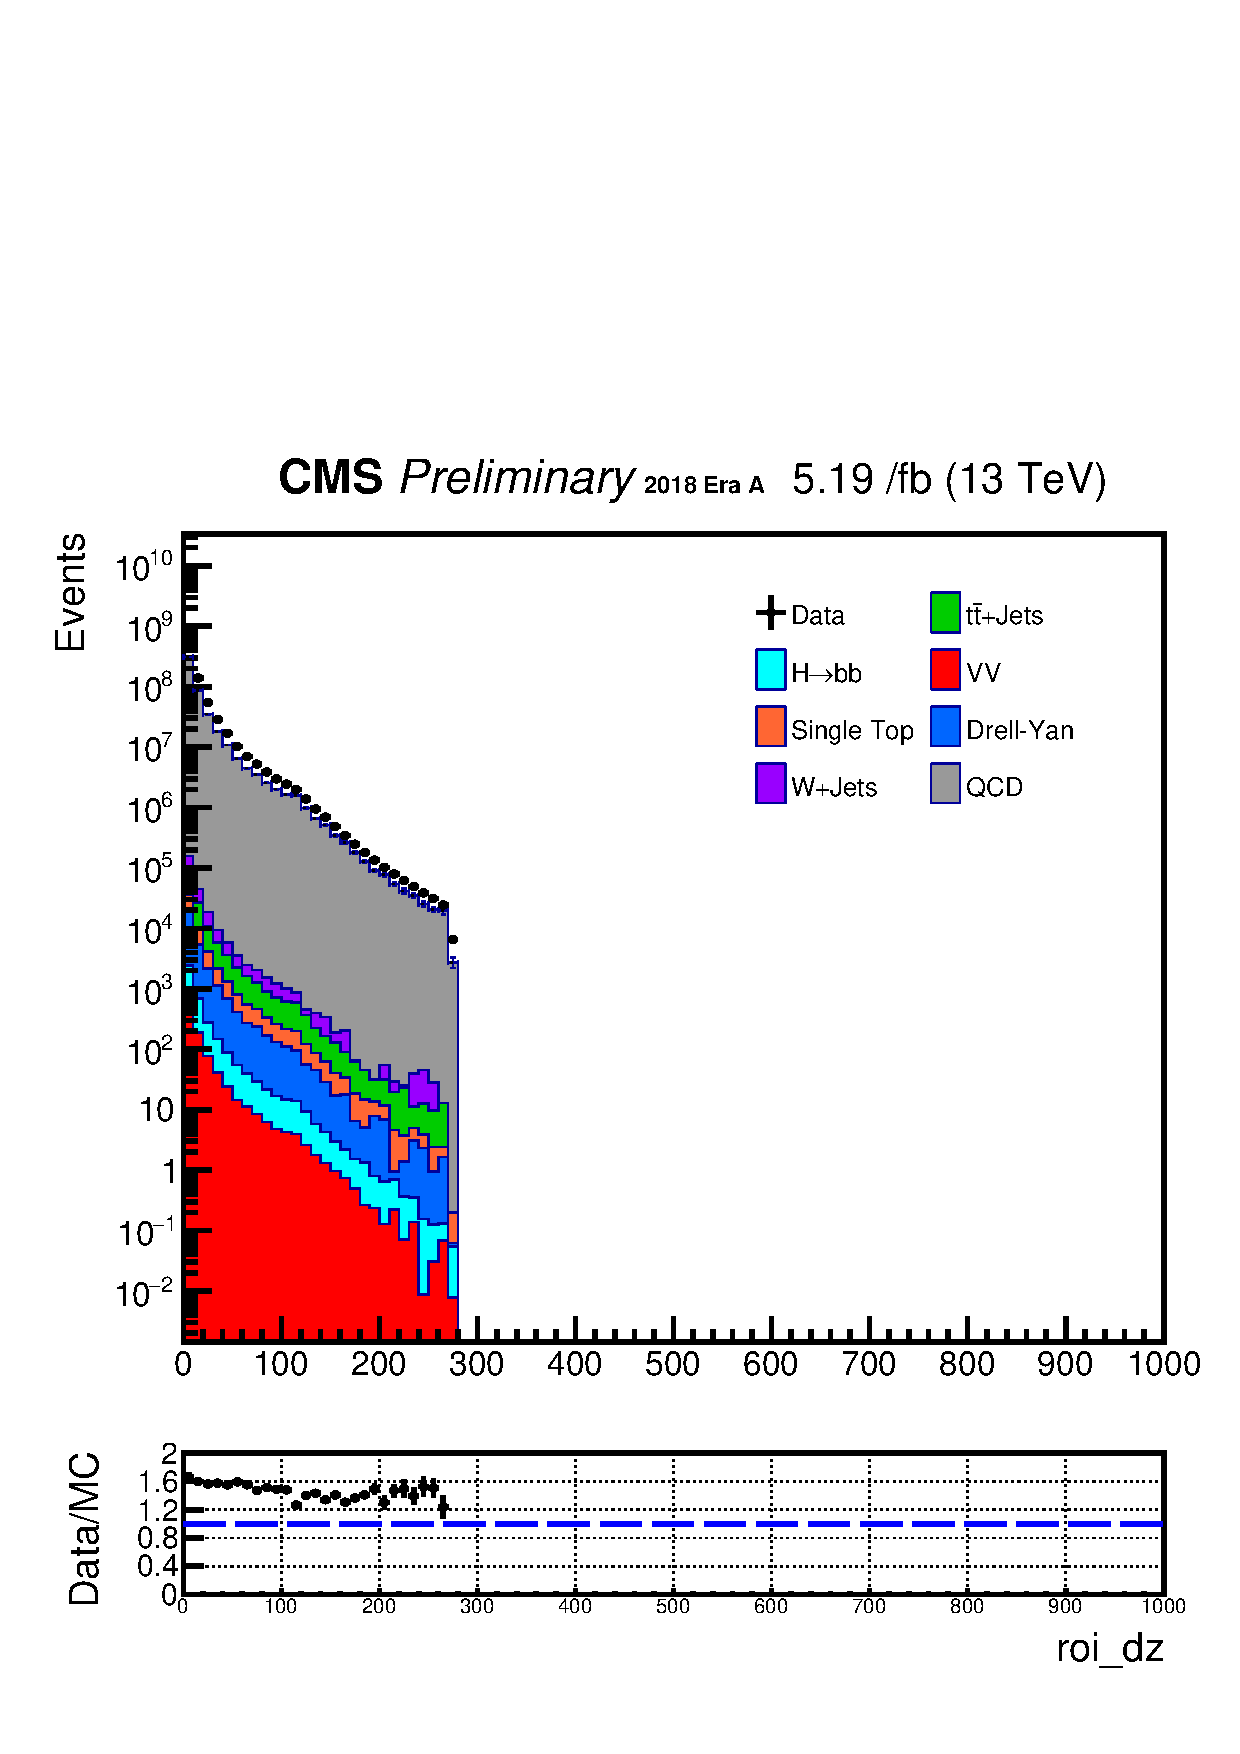
\includegraphics[width=0.47\linewidth]{figs/Data_log_Oct6ANVars_MS-15_ctauS-10_roi_dz.pdf}
%\end{figure}
%
%\begin{figure}[h!]
%  \caption{Data/MC of number of fitted vertices in ROI and nember of annulus tracks in ROI}
%  \label{fig:2ROIs}
%  \centering
%  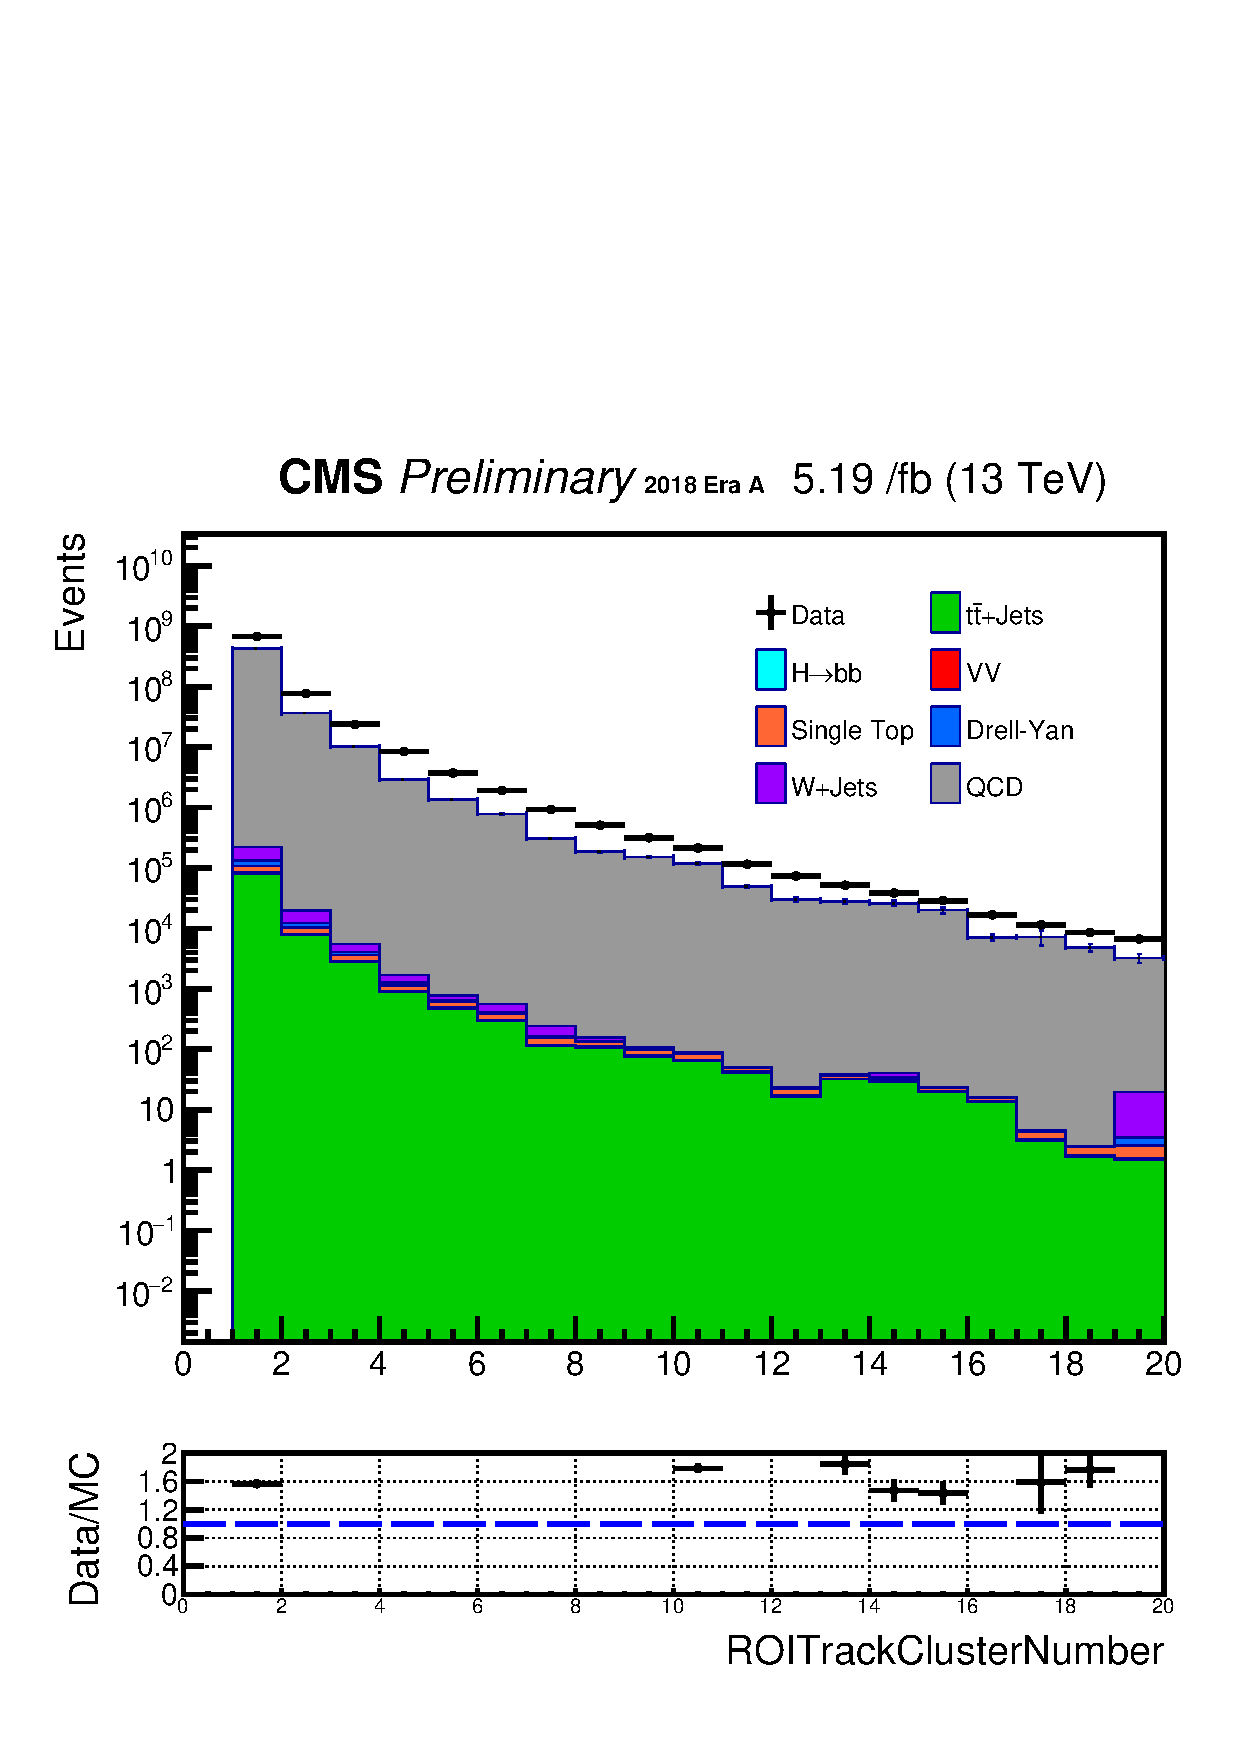
\includegraphics[width=0.47\linewidth]{figs/Data_log_Oct6ANVars_MS-15_ctauS-10_ROITrackClusterNumber.pdf}
%  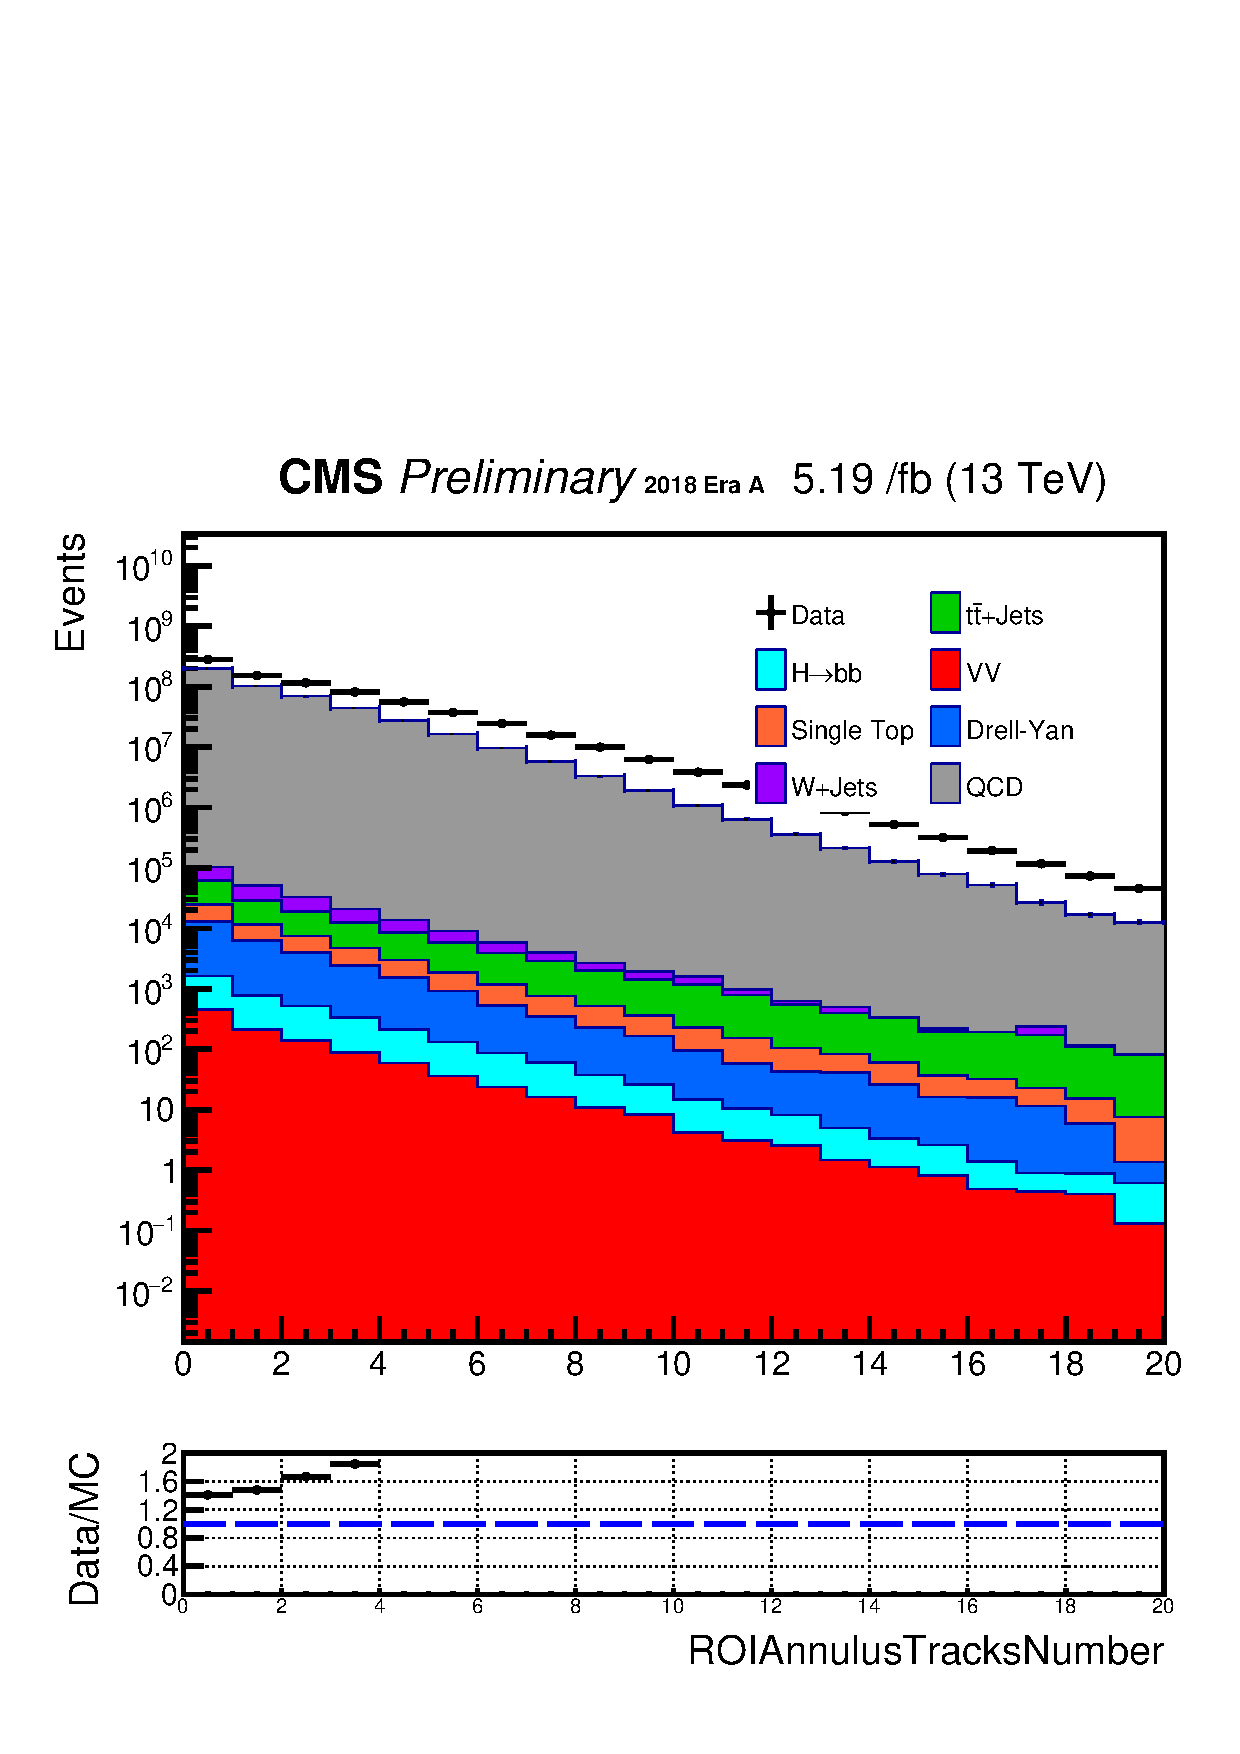
\includegraphics[width=0.47\linewidth]{figs/Data_log_Oct6ANVars_MS-15_ctauS-10_ROIAnnulusTracksNumber.pdf}
%\end{figure}
